\documentclass[12pt,a4paper]{report}

% ====================================================================
% MARGINS & TYPOGRAPHY SPECIFICATIONS (AS PER COLLEGE GUIDELINES)
% Left: 1.5 in, Top: 1.0 in, Bottom: 1.0 in, Right: 1.0 in
% Font: Times New Roman, 12 pt, 1.5 Line Spacing
% ====================================================================
\usepackage[left=1.5in, right=1.0in, top=1.0in, bottom=1.0in]{geometry}
\usepackage{times}
\usepackage{setspace}
\onehalfspacing

\usepackage[utf8]{inputenc}
\usepackage{graphicx}
\graphicspath{{./}{../}}
\usepackage{amsmath,amssymb,amsfonts}
\usepackage{booktabs}
\usepackage{longtable}
\usepackage{array}
\usepackage{caption}
\usepackage{subcaption}
\usepackage{titlesec}
\usepackage{fancyhdr}
\usepackage{tocloft}
\usepackage[hidelinks]{hyperref}
\usepackage{cite}

% Captions formatting: Tables on TOP, Figures on BOTTOM
\captionsetup[table]{position=top, labelfont=bf, textfont=normalfont, skip=6pt}
\captionsetup[figure]{position=bottom, labelfont=bf, textfont=normalfont, skip=6pt}

% Chapter headings formatting
\titleformat{\chapter}[DISPLAY]
  {\normalfont\Large\bfseries\centering}{\chaptertitlename\ \thechapter}{12pt}{\Large\MakeUppercase}
\titlespacing*{\chapter}{0pt}{0pt}{20pt}

\titleformat{\section}
  {\normalfont\large\bfseries}{\thesection}{1em}{}
\titleformat{\subsection}
  {\normalfont\normalsize\bfseries}{\thesubsection}{1em}{}

% Header and Footer
\pagestyle{fancy}
\fancyhf{}
\fancyhead[R]{\thepage}
\renewcommand{\headrulewidth}{0pt}

\begin{document}

% ====================================================================
% 1. COVER PAGE & TITLE PAGE
% ====================================================================
\begin{titlepage}
    \centering
    \vspace*{0.5cm}
    {\large \bfseries WASSERSTEIN-GUIDED DYNAMIC LLM KNOWLEDGE DISTILLATION TRANSFER FOR EMOTION-AWARE AUTOMATIC SPEECH RECOGNITION \par}
    
    \vspace{1.5cm}
    {\normalsize \textbf{A PROJECT REPORT} \par}
    \vspace{0.3cm}
    {\normalsize \textit{Submitted by} \par}
    \vspace{0.6cm}
    
    {\large \bfseries DEEPAK R.G \quad (951421205011) \par}
    \vspace{0.2cm}
    {\large \bfseries PURUSHOTHAMAN V \quad (951421205035) \par}
    
    \vspace{1.5cm}
    {\normalsize \textit{in partial fulfillment for the award of the degree of} \par}
    \vspace{0.4cm}
    {\large \bfseries BACHELOR OF TECHNOLOGY \par}
    \vspace{0.2cm}
    {\normalsize in \par}
    \vspace{0.2cm}
    {\large \bfseries ARTIFICIAL INTELLIGENCE AND DATA SCIENCE \par}
    
    \vfill
    \IfFileExists{mepco_logo.png}{\includegraphics[width=3.2cm]{mepco_logo.png}}{\IfFileExists{../mepco_logo.png}{\includegraphics[width=3.2cm]{../mepco_logo.png}}{\vspace{2.5cm}}} \par
    \vspace{0.5cm}
    
    {\large \bfseries DEPARTMENT OF ARTIFICIAL INTELLIGENCE AND DATA SCIENCE \par}
    \vspace{0.2cm}
    {\large \bfseries MEPCO SCHLENK ENGINEERING COLLEGE \par}
    {\normalsize \textbf{(An Autonomous Institution, Affiliated to Anna University, Chennai)} \par}
    {\normalsize \textbf{SIVAKASI - 626 005, TAMIL NADU, INDIA} \par}
    \vspace{0.5cm}
    {\normalsize \bfseries APRIL 2026 \par}
\end{titlepage}

% ====================================================================
% 2. BONAFIDE CERTIFICATE (14pt, Double Spacing)
% ====================================================================
\newpage
\thispagestyle{empty}
\begin{doublespacing}
\begin{center}
    {\fontsize{14pt}{18pt}\selectfont \bfseries MEPCO SCHLENK ENGINEERING COLLEGE, SIVAKASI \par}
    {\fontsize{12pt}{16pt}\selectfont \textbf{(An Autonomous Institution, Affiliated to Anna University, Chennai)} \par}
    \vspace{0.4cm}
    {\fontsize{14pt}{18pt}\selectfont \bfseries DEPARTMENT OF ARTIFICIAL INTELLIGENCE AND DATA SCIENCE \par}
    \vspace{0.8cm}
    {\fontsize{14pt}{18pt}\selectfont \bfseries BONAFIDE CERTIFICATE \par}
\end{center}

\vspace{0.4cm}
\noindent Certified that this project report titled \textbf{``WASSERSTEIN-GUIDED DYNAMIC LLM KNOWLEDGE DISTILLATION TRANSFER FOR EMOTION-AWARE AUTOMATIC SPEECH RECOGNITION''} is the bonafide work of \textbf{DEEPAK R.G} and \textbf{PURUSHOTHAMAN V} who carried out the project work under my supervision.

\vspace{2.5cm}

\noindent
\begin{tabular}{p{7.5cm}p{7.5cm}}
    \textbf{SIGNATURE} & \textbf{SIGNATURE} \\[1.8cm]
    \textbf{Dr. K. THIRUMOORTHY, B.E., M.E., Ph.D.} & \textbf{HEAD OF THE DEPARTMENT} \\
    \textbf{SUPERVISOR} & Department of Artificial Intelligence \\
    Professor, & and Data Science, \\
    Department of Artificial Intelligence & Mepco Schlenk Engineering College, \\
    and Data Science, & Sivakasi - 626 005. \\
    Mepco Schlenk Engineering College, & \\
    Sivakasi - 626 005. & 
\end{tabular}

\vspace{1.0cm}
\noindent Submitted for the Project Viva-Voce examination held on \rule{4.5cm}{0.4pt}.

\vspace{1.5cm}
\noindent
\begin{tabular}{p{7.5cm}p{7.5cm}}
    \textbf{INTERNAL EXAMINER} & \textbf{EXTERNAL EXAMINER}
\end{tabular}
\end{doublespacing}

% ====================================================================
% 3. ABSTRACT (1 Page Synopsis)
% ====================================================================
\newpage
\pagenumbering{roman}
\setcounter{page}{3}
\begin{center}
    {\Large \bfseries ABSTRACT \par}
\end{center}
\vspace{0.5cm}

Automatic Speech Recognition (ASR) deployed in real-time edge environments faces severe bottlenecks in maintaining transcription fidelity under emotional stress while capturing paralinguistic tone. Although foundational causal Large Language Models (LLMs) encode rich linguistic syntax and world knowledge, distilling this knowledge to compact acoustic front-ends suffers from an extreme $125\times$ vocabulary cardinality mismatch ($|\mathcal{V}_{\text{teacher}}| = 128{,}256$ vs $|\mathcal{V}_{\text{student}}| = 1{,}024$), rendering standard Kullback-Leibler (KL) divergence fundamentally inapplicable. Furthermore, non-autoregressive Connectionist Temporal Classification (CTC) decoders frequently collapse into degenerate blank-token attractors due to a 14:1 acoustic-phoneme frame oversampling disparity.

To eliminate these theoretical and operational limitations, this project develops an end-to-end multi-task framework that transfers continuous causal linguistic priors from a frozen $1.2\text{B}$-parameter foundation LLM into an ultra-compact $12.55\text{M}$-parameter Conformer student via entropic Sinkhorn-Wasserstein Optimal Transport (OT). By modeling cross-vocabulary alignment as continuous probability mass transportation over cosine-normalized semantic manifolds, the system bypasses heuristic string discard rules, eliminates heavy projection layers, and acts as an implicit lexical anchor that suppresses blank over-allocation. The unified latent representation simultaneously powers non-autoregressive transcription and 4-class Speech Emotion Recognition (SER) via decoupled prediction heads.

Extensive empirical evaluations across the LibriSpeech and IEMOCAP corpora confirm that the proposed $12.55\text{M}$ Conformer achieves a Word Error Rate (WER) of 37.5\% on clean speech (a 45.2\% relative improvement over unregularized CTC) and an Unweighted Accuracy (UA) of 59.97\% on held-out emotional dialogue, while operating at a Real-Time Factor of $\text{RTF}_{\text{CPU}} = 0.08$ on commodity CPU hardware ($12.5\times$ faster than real-time). Crucially, deploying the distilled model as an automated adjudicator across 2,507 ambiguous non-consensus human utterances from the IEMOCAP corpus yields a 72.72\% Human-AI consensus rate, resolving real-world human perceptual ambiguity.

% ====================================================================
% 4. PRELIMINARY LISTS
% ====================================================================
\newpage
\tableofcontents

\newpage
\listoftables

\newpage
\listoffigures

\newpage
\chapter*{LIST OF SYMBOLS, ABBREVIATIONS AND NOMENCLATURE}
\addcontentsline{toc}{chapter}{LIST OF SYMBOLS, ABBREVIATIONS AND NOMENCLATURE}

\begin{longtable}{p{2.5cm}p{12cm}}
\textbf{AED} & Attention-based Encoder-Decoder \\
\textbf{ASR} & Automatic Speech Recognition \\
\textbf{BPE} & Byte-Pair Encoding \\
\textbf{CER} & Character Error Rate \\
\textbf{CMVN} & Cepstral Mean and Variance Normalization \\
\textbf{CTC} & Connectionist Temporal Classification \\
\textbf{EOT} & Entropic Optimal Transport \\
\textbf{GLU} & Gated Linear Unit \\
\textbf{HMM} & Hidden Markov Model \\
\textbf{IEMOCAP} & Interactive Emotional Dyadic Motion Capture \\
\textbf{KD} & Knowledge Distillation \\
\textbf{KL} & Kullback-Leibler (Divergence) \\
\textbf{LLM} & Large Language Model \\
\textbf{LOSO} & Leave-One-Session-Out \\
\textbf{MHSA} & Multi-Head Self-Attention \\
\textbf{MLP} & Multi-Layer Perceptron \\
\textbf{OT} & Optimal Transport \\
\textbf{PEFT} & Parameter-Efficient Fine-Tuning \\
\textbf{RTF} & Real-Time Factor \\
\textbf{SDG} & Sustainable Development Goals \\
\textbf{SER} & Speech Emotion Recognition \\
\textbf{SWD} & Sinkhorn-Wasserstein Distance \\
\textbf{UA} & Unweighted Accuracy \\
\textbf{WA} & Weighted Accuracy \\
\textbf{WER} & Word Error Rate \\
$\mathcal{V}_{\text{teacher}}$ & Teacher Vocabulary Lexicon ($128{,}256$ subwords) \\
$\mathcal{V}_{\text{student}}$ & Student Subword Vocabulary ($1{,}024$ BPE tokens) \\
$C_{ij}$ & Ground Cost Metric between token $i$ and token $j$ \\
$P^*$ & Optimal Transport Coupling Plan Matrix \\
$\gamma$ & Entropic Regularization Coefficient ($\gamma = 0.10$) \\
$\mathcal{L}_{\text{total}}$ & Composite Multi-Task Optimization Loss \\
$\lambda_{\text{OT}}$ & Optimal Transport Distillation Weight ($\lambda_{\text{OT}} = 0.1$) \\
$\lambda_{\text{emo}}$ & Affective Classification Weight ($\lambda_{\text{emo}} = 0.2$) \\
$\pi_\emptyset$ & CTC Null/Blank Token Attractor Probability \\
\end{longtable}

% ====================================================================
% MAIN CHAPTERS (ARABIC NUMERALS)
% ====================================================================
\newpage
\pagenumbering{arabic}
\setcounter{page}{1}

\chapter{INTRODUCTION}
\label{ch:intro}

\section{Overview of Spoken Language Processing}
Spoken language processing constitutes one of the foundational frontiers in artificial intelligence, bridging human acoustic communication and computational linguistic intelligence. The primary objective of Automatic Speech Recognition (ASR) is to transform continuous, time-varying acoustic speech waveforms into accurate orthographic textual representations. Concurrently, Speech Emotion Recognition (SER) endeavors to decode paralinguistic and affective cues—such as anger, joy, sadness, and neutral communicative composure—embedded within the subtle prosodic excursions, pitch modulations, and formant trajectories of human speech. 

In conventional spoken language interfaces, speech transcription and emotion recognition have historically been treated as distinct, disjoint engineering tasks. Acoustic models dedicated to ASR prioritize phoneme discrimination while treating emotional modulations as non-stationary acoustic noise that should be normalized or suppressed. Conversely, affective computing systems frequently operate on isolated acoustic feature descriptors or post-transcription sentiment analysis, losing the intrinsic subword acoustic alignments that govern emotional expression. Developing a unified architecture capable of joint acoustic transcription and paralinguistic state estimation represents a vital leap toward natural, empathetic human-computer interaction.

\section{The Paradox of Modern Foundation Models}
The landscape of natural language processing has undergone an extraordinary revolution driven by the emergence of generative, autoregressive Large Language Models (LLMs). Contemporary foundation models, trained on trillions of textual tokens, exhibit unmatched syntactic understanding, long-range contextual reasoning, and encyclopedic semantic grounding. Consequently, integrating this immense linguistic competence into acoustic speech recognition decoders has become an active pursuit.

However, a severe architectural paradox impedes the edge deployment of foundation-model-powered speech decoders:
\begin{enumerate}
    \item \textbf{Computational Footprint and Memory Wall:} Multi-billion parameter generative decoders require tens of gigabytes of volatile memory and immense floating-point operations per second. Deploying such cumbersome decoders on resource-constrained embedded edge devices, mobile processors, or in low-latency voice assistants creates prohibitive computational overhead, high energy consumption, and intolerable inference latency.
    \item \textbf{Vocabulary Cardinality and Geometry Mismatch:} Foundational language models operate over massive subword vocabularies optimized for global text generation ($|\mathcal{V}_{\text{teacher}}| > 120{,}000$ subwords). In contrast, efficient non-autoregressive acoustic decoders achieve optimal real-time performance with compact vocabularies ($|\mathcal{V}_{\text{student}}| \approx 1{,}000$ to $5{,}000$ tokens). Direct distribution matching via classical knowledge transfer is fundamentally ill-posed when teacher and student probability simplices occupy mutually disjoint categorical spaces.
\end{enumerate}

\section{Problem Statement}
When standard knowledge distillation paradigms are applied across heterogeneous acoustic and linguistic architectures, three major structural failure modes emerge:
\begin{itemize}
    \item \textbf{Infeasibility of Divergence-Based Distillation:} Conventional knowledge distillation relies on Kullback-Leibler (KL) divergence or mean-squared error over categorical output logits. These measures strictly require an isomorphic vocabulary space ($\mathcal{V}_{\text{teacher}} = \mathcal{V}_{\text{student}}$). When vocabularies diverge in cardinality and tokenization boundaries, KL divergence collapses because probability distributions share no common geometric support.
    \item \textbf{Degenerate CTC Blank Attractor Collapse:} Non-autoregressive acoustic decoders trained via Connectionist Temporal Classification (CTC) suffer from a severe frame-to-phoneme oversampling disparity (typically 14:1). Under standard optimization, decoders fall into a pathological local minimum known as \textit{Blank Collapse}, where the network assigns over 90\% of its probability mass to the null transition token ($\pi_\emptyset$), virtually choking valid phonetic emission.
    \item \textbf{Loss of Nuanced Paralinguistic Cues:} Standard acoustic distillation techniques fail to preserve affective prosody, discarding expressive speech inflections and emotional nuance. Furthermore, ambiguous human conversations—where human annotators themselves disagree on emotional categories—are routinely discarded by existing pipelines, limiting real-world robustness.
\end{itemize}

\section{Aim and Objectives of the Project}

\subsection{Project Aim}
The principal aim of this project is to develop an ultra-compact, end-to-end multi-task speech framework that transfers rich linguistic priors from a high-capacity generative language model into an efficient acoustic encoder via Optimal Transport, concurrently achieving robust speech recognition and speech emotion classification with real-time edge viability.

\subsection{Key Objectives}
To accomplish this aim, the following specific objectives are established:
\begin{enumerate}
    \item To design a decimated, lightweight 6-layer Conformer acoustic student backbone ($12.55\text{M}$ parameters) integrated with $4\times$ 2D-convolutional subsampling to neutralize CTC blank collapse while preserving temporal acoustic resolution.
    \item To formulate a continuous cross-vocabulary distillation bridge using entropic Sinkhorn-Wasserstein Optimal Transport (OT), allowing probability mass to be transported smoothly across mismatched token vocabularies ($|\mathcal{V}_{\text{teacher}}| = 128{,}256$ vs $|\mathcal{V}_{\text{student}}| = 1{,}024$) without heuristic token pruning.
    \item To implement a frozen foundation teacher dynamic based on an autoregressive language model, ensuring zero runtime LLM memory consumption during edge execution.
    \item To construct dual decoupled prediction heads—a Connectionist Temporal Classification transcription head and a temporal-mean-pooled affective classification head—optimized via a joint composite loss function.
    \item To empirically validate the framework on the benchmark LibriSpeech and IEMOCAP corpora, evaluating Word Error Rate (WER), Character Error Rate (CER), Weighted Accuracy (WA), Unweighted Accuracy (UA), and edge Real-Time Factor (RTF).
    \item To deploy the trained multi-task student as an automated impartial adjudicator over 2,507 ambiguous non-consensus human utterances from the IEMOCAP corpus to resolve human perceptual disagreement.
\end{enumerate}

\section{Organization of the Report}
The remainder of this project report is systematically structured into the following chapters:
\begin{itemize}
    \item \textbf{Chapter 2 (Literature Survey):} Presents an in-depth review of existing acoustic modeling paradigms, Connectionist Temporal Classification, knowledge distillation methodologies, and five contemporary base papers, identifying critical research gaps.
    \item \textbf{Chapter 3 (System Study and Feasibility Analysis):} Analyzes existing speech distillation workflows, details technical, operational, and economic feasibility, evaluates the LibriSpeech and IEMOCAP datasets, and presents a SWOT analysis.
    \item \textbf{Chapter 4 (System Design):} Elaborates the mathematical architecture of the Conformer student, generative teacher, entropic Sinkhorn Optimal Transport formulation, solved numerical matrix illustration, and dual task heads.
    \item \textbf{Chapter 5 (System Implementation):} Formulates the end-to-end training pipeline, multi-stage distillation workflow, dynamic key-padding masking, and two-pass hybrid decoding strategy.
    \item \textbf{Chapter 6 (Results and Discussion):} Provides quantitative empirical benchmarks across clean and emotional speech, extensive ablation studies, latency profiles, and the qualitative resolution of ambiguous human discourse.
    \item \textbf{Chapter 7 (Conclusion and Future Enhancement):} Summarizes the primary contributions of the study and outlines promising directions for future research.
\end{itemize}

\chapter{LITERATURE SURVEY}
\label{ch:literature}

\section{Evolution of Acoustic Modeling Paradigms}
The field of Automatic Speech Recognition (ASR) has undergone continuous architectural transformation over the past three decades. Early speech processing systems relied primarily on hybrid architectures combining Hidden Markov Models with Gaussian Mixture Models (HMM-GMM) to model temporal sequence transitions and spectral emission probabilities. With the advent of deep learning, Deep Neural Networks (HMM-DNN) replaced GMMs, yielding noticeable gains in phoneme recognition. Nevertheless, these hybrid frameworks remained heavily burdened by the necessity for complex, multi-stage pipelines requiring explicit frame-level phonetic alignments, forced alignment algorithms, and decoupled pronunciation lexicons.

To alleviate the compounding errors of multi-stage pipelines, the community transitioned toward end-to-end (E2E) sequence-to-sequence formulations. Notable milestones include:
\begin{enumerate}
    \item \textbf{Attention-Based Encoder-Decoder (AED) Models:} Exemplified by architectures such as Listen, Attend and Spell (LAS) \cite{chan2016listen}, AED models decouple acoustic encoding from autoregressive linguistic generation via cross-attention mechanisms. While effective at capturing long-term dependencies, AED architectures suffer from label exposure bias, hallucination phenomena during extended acoustic pauses, and quadratic computational complexity $\mathcal{O}(T^2)$ during decoding, making real-time streaming infeasible.
    \item \textbf{Recurrent Neural Network Transducers (RNN-T):} Formulated by Graves \cite{graves2012sequence}, RNN-T models decouple acoustic feature encoding and linguistic sequence prediction into separate sub-networks merged via a joint network. Although RNN-T operates in a streaming fashion, calculating the forward-backward variable lattice over the 3D tensor $\mathcal{O}(B \times T \times U \times |\mathcal{V}|)$ requires massive GPU memory during training, while its autoregressive prediction network creates sequential decoding bottlenecks.
    \item \textbf{Self-Attention Transformers and the Conformer Paradigm:} Vaswani et al. \cite{vaswani2017attention} introduced the Transformer architecture, replacing recurrent units with Multi-Head Self-Attention (MHSA). While Transformers excel at global context aggregation, speech signals exhibit localized inductive structures: formant resonance transitions and vocal tract dynamics occur over short time spans (10 to 50 ms). To bridge global contextual modeling with localized spatial filtering, Gulati et al. \cite{gulati2020conformer} introduced the Conformer architecture. By interleaving depthwise separable convolutions with self-attention inside a Macaron-style feed-forward backbone, the Conformer establishes superior parameter efficiency and acoustic representation fidelity.
\end{enumerate}

\section{Connectionist Temporal Classification and Blank Collapse}
Connectionist Temporal Classification (CTC), introduced by Graves et al. \cite{graves2006connectionist}, eliminated the requirement for pre-segmented training alignments by introducing an auxiliary null transition symbol, termed the blank token ($\pi_\emptyset$). CTC evaluates the conditional probability of a target subword sequence $Y = (y_1, \dots, y_U)$ given an acoustic sequence $X = (x_1, \dots, x_T)$ by marginalizing across all valid valid alignment paths $\pi \in \mathcal{B}^{-1}(Y)$:
\begin{equation}
    P(Y \mid X) = \sum_{\pi \in \mathcal{B}^{-1}(Y)} \prod_{t=1}^T P(\pi_t \mid x_t)
\end{equation}
where $\mathcal{B}$ denotes the sequence collapse operator that removes consecutive repeated labels and deletes blank emissions.

Despite the advantage of non-autoregressive parallel decoding during inference, pure CTC models operate under a conditional independence assumption: labels emitted at time frame $t$ are statistically independent of labels emitted at time $t-1$, conditioned on the entire acoustic input $X$. In practical acoustic modeling, the acoustic frame sampling rate drastically exceeds the phoneme emission rate, typically yielding a 14:1 oversampling ratio. Consequently, unregularized CTC networks converge to a trivial degenerate state known as \textit{Blank Collapse}, wherein the model outputs blank tokens for more than 90\% of the time steps, collapsing valid character emissions into sharp, highly fragile spike intervals.

\section{Knowledge Distillation Paradigms in Speech Processing}
Knowledge Distillation (KD), pioneered by Hinton et al., provides an elegant framework for transferring dark knowledge—soft contextual class probabilities—from a high-capacity teacher network to a resource-constrained student. In speech processing, distillation protocols have expanded across three primary paradigms:
\begin{enumerate}
    \item \textbf{Logit-Based Distillation:} The student matches the temperature-scaled posterior class probabilities of the teacher by minimizing Kullback-Leibler (KL) divergence. However, this approach presupposes an isomorphic vocabulary space ($\mathcal{V}_{\text{teacher}} = \mathcal{V}_{\text{student}}$), failing when vocabulary tokenizers differ.
    \item \textbf{Intermediate Feature Distillation:} The student minimizes the mean-squared error or cosine distance between intermediate hidden representation layers. This requires matching or projecting latent feature dimensions, often inducing architectural rigidity.
    \item \textbf{Cross-Modal and Optimal Transport Distillation:} Emerging techniques map representations across disparate structural spaces by formulating probability mass transportation over continuous semantic spaces, circumventing discrete token mismatch.
\end{enumerate}

\section{Detailed Survey of Contemporary Base Works}

\subsection{Base Paper 1: Distilling Knowledge of LLMs for ASR}
\textbf{Citation:} Hayato Futami and Tatsuya Kawahara (2026), `Distilling the Knowledge of LLMs for Automatic Speech Recognition', \textit{IEEE/ACM Transactions on Audio, Speech, and Language Processing}, Vol. 34, pp. 2962--2971.

\subsubsection{Methodology Overview}
Futami and Kawahara investigated the transfer of linguistic knowledge from autoregressive Large Language Models into compact ASR decoders. To bridge the directional discrepancy between causal LLM decoders and non-causal speech decoders, the authors proposed a Pseudo-Bidirectional Knowledge Distillation (PBKD) framework. Contextual representations were extracted by conditioning the LLM on future lookahead text windows. To address the vocabulary mismatch between the LLM tokenizer ($|\mathcal{V}_{\text{LM}}| \approx 32\text{k}$) and the ASR tokenizer ($|\mathcal{V}_{\text{ASR}}| \approx 1\text{k}$), the authors employed a normalized Levenshtein edit-distance string alignment heuristic.

\subsubsection{Key Advantages (Pros)}
\begin{itemize}
    \item Successfully demonstrated that causal generative LLMs can serve as effective linguistic teachers for non-causal speech decoders via pseudo-bidirectional windowing.
    \item Formulated an initial heuristic solution to the vocabulary discrepancy problem without requiring full LLM fine-tuning.
\end{itemize}

\subsubsection{Critical Drawbacks and Limitations (Cons)}
\begin{itemize}
    \item \textbf{Rigid Discard Thresholds:} The edit-distance heuristic relies on a hard threshold ($d \le 0.2$). Subwords that fail exact one-to-one mapping (such as multi-token subword splits like ``observing'' $\to$ ``obs'' + ``erving'') are completely discarded from distillation supervision, losing vital lexical information.
    \item \textbf{Computational Inefficiency:} Re-scoring candidate tokens dynamically using edit distance introduces high algorithmic overhead during training batch compilation.
    \item \textbf{Narrow Candidate Truncation:} The alignment is restricted to the top-512 most likely candidate words at each step, preventing the student from acquiring full semantic distribution tails.
\end{itemize}

\subsection{Base Paper 2: Multimodal Emotion Recognition with LoRA}
\textbf{Citation:} Feng Liu, Ziwang Fu, and Yunlong Wang (2025), `Reward-Based Gradient Modulation for Multimodal Emotion Recognition with LoRA', \textit{IEEE Transactions on Computational Social Systems}, Vol. 12, No. 5, pp. 3301--3310.

\subsubsection{Methodology Overview}
Liu et al. explored Parameter-Efficient Fine-Tuning (PEFT) for multimodal emotion recognition across speech, text, and visual modalities. To adapt pre-trained transformer backbones without destroying foundational representations, Low-Rank Adaptation (LoRA) adapters were injected into multi-head attention projection layers. The authors introduced a reward-based gradient modulation strategy to dynamically reweight gradient updates across dominant and sluggish modalities during backpropagation.

\subsubsection{Key Advantages (Pros)}
\begin{itemize}
    \item Achieved high parameter efficiency by freezing base foundation weights ($W_0$) and optimizing only low-rank matrices ($A$ and $B$).
    \item Alleviated modality suppression by actively balancing gradient competition between textual and acoustic channels.
    \item Prevented catastrophic forgetting of pre-trained linguistic hierarchies.
\end{itemize}

\subsubsection{Critical Drawbacks and Limitations (Cons)}
\begin{itemize}
    \item \textbf{Uniform Feature Treatment:} The model treats audio and video streams identically within feature extraction pipelines, neglecting the localized temporal dynamics unique to acoustic speech formants.
    \item \textbf{Absence of Noise Handling:} Lacks explicit acoustic noise calibration or frame subsampling, rendering the model vulnerable to pitch jitter and environmental noise.
    \item \textbf{Single-Task Restriction:} Focuses exclusively on emotion classification and cannot perform speech transcription.
\end{itemize}

\subsection{Base Paper 3: Steering Language Models to Stable Speech Emotion Recognition}
\textbf{Citation:} Zhixian Zhao, Xinfa Zhu, Xinsheng Wang, Shuiyuan Wang, Xuelong Geng, Wenjie Tian, and Lei Xie (2026), `Steering Language Model to Stable Speech Emotion Recognition via Contextual Perception and Chain of Thought', \textit{IEEE/ACM Transactions on Audio, Speech, and Language Processing}, Vol. 34, pp. 3110--3123.

\subsubsection{Methodology Overview}
Zhao et al. formulated a framework using generative LLMs for conversational emotion recognition by guiding the model through a Chain-of-Thought (CoT) reasoning mechanism. The architecture integrates dual contextual perception, combining audio tone features with dialogue discourse transcripts to infer emotional shifts.

\subsubsection{Key Advantages (Pros)}
\begin{itemize}
    \item Effectively suppresses hallucination in LLM-based affective reasoning by grounding predictions on acoustic prosody.
    \item Captures dual contextual perception by jointly reasoning over speaker tone and semantic content.
\end{itemize}

\subsubsection{Critical Drawbacks and Limitations (Cons)}
\begin{itemize}
    \item \textbf{Heavy Resource Footprint:} Requires multi-billion parameter LLMs during active inference, requiring high GPU memory and generating high latency unsuitable for edge deployment.
    \item \textbf{Minority Class Breakdown:} Suffers severe accuracy degradation on minority emotion categories (fear and disgust dropped below 20\% accuracy).
\end{itemize}

\subsection{Base Paper 4: Evaluating Speech Emotion Recognition on IEMOCAP}
\textbf{Citation:} Nikolaos Antoniou, Athanasios Katsamanis, Theodoros Giannakopoulos, and Shrikanth Narayanan (2023), `Designing and Evaluating Speech Emotion Recognition Systems: A Reality Check Case Study with IEMOCAP', \textit{Language Resources and Evaluation}, Vol. 57, pp. 1105--1132.

\subsubsection{Methodology Overview}
Antoniou et al. conducted an empirical audit of Speech Emotion Recognition systems evaluated on the benchmark IEMOCAP dataset. The authors investigated widespread experimental flaws in the literature, including speaker contamination across training and test splits, arbitrary class merging, and the exclusion of challenging emotional categories.

\subsubsection{Key Findings and Recommendations}
\begin{itemize}
    \item Standardized the requirement for strict 5-fold Leave-One-Session-Out (LOSO) cross-validation to evaluate speaker-independent generalization.
    \item Demonstrated that evaluating models without speaker separation yields severely overfitted, non-generalizable performance metrics.
    \item Highlighted the necessity of reporting both Weighted Accuracy (WA) and Unweighted Accuracy (UA) to account for natural emotional class imbalances.
\end{itemize}

\subsection{Base Paper 5: Continual Learning in ASR via Singular Value Tuning}
\textbf{Citation:} Steven Vander Eeckt and Hugo Van hamme (2026), `Efficient Rehearsal for Continual Learning in ASR via Singular Value Tuning', \textit{IEEE/ACM Transactions on Audio, Speech, and Language Processing}, Vol. 34, pp. 1420--1432.

\subsubsection{Methodology Overview}
Eeckt and Van hamme investigated parameter-efficient continual learning in ASR architectures. To adapt acoustic decoders to new acoustic domains without catastrophic forgetting, the authors proposed Singular Value Tuning (SVT), wherein singular values of weight matrices are adapted while singular vectors remain frozen.

\subsubsection{Key Advantages (Pros)}
\begin{itemize}
    \item Exceptional parameter compactness and memory economy during incremental adaptation.
    \item Mitigates overfitting on small acoustic subsets.
\end{itemize}

\subsubsection{Critical Drawbacks and Limitations (Cons)}
\begin{itemize}
    \item Tuning only singular values restricts representation capacity when bridging massive cross-modal vocabulary disparities.
    \item High hyperparameter sensitivity when scaling to multilingual or multi-task acoustic pipelines.
\end{itemize}

\section{Summary of Research Gaps and Proposed Interventions}
Table \ref{tab:lit_comparison} synthesizes the key attributes, methodologies, and limitations of existing speech distillation frameworks in comparison to our proposed Wasserstein-guided multi-task system.

\begin{table}[htbp]
\centering
\caption{Comprehensive Comparison of Literature Survey Base Works and Proposed System}
\label{tab:lit_comparison}
\small
\begin{tabular}{p{3.2cm}p{3.0cm}p{4.2cm}p{3.6cm}}
\toprule
\textbf{Research Work} & \textbf{Core Methodology} & \textbf{Identified Limitations} & \textbf{Proposed Framework Solution} \\
\midrule
Futami \& Kawahara (2026) \cite{futami2026distilling} & Edit-distance string alignment from LLM & Rigid discard threshold ($d \le 0.2$), discards multi-token splits & Continuous entropic Optimal Transport (Zero token discard) \\
\addlinespace
Liu et al. (2025) \cite{liu2025reward} & PEFT LoRA for multimodal emotion & Single-task (SER only), no acoustic temporal subsampling & Joint multi-task (ASR + SER), 4x 2D-Conv subsampling \\
\addlinespace
Zhao et al. (2026) \cite{zhao2026steering} & Contextual Chain-of-Thought in LLM & Prohibitive inference latency, requires LLM at test time & Frozen teacher; compact 12.55M student with zero runtime LLM \\
\addlinespace
Antoniou et al. (2023) \cite{antoniou2023designing} & IEMOCAP evaluation audit & Discards ambiguous non-consensus ($xxx$) utterances & Automated AI adjudicator yielding 72.72\% consensus \\
\addlinespace
Eeckt \& Hamme (2026) \cite{eeckt2026efficient} & Singular Value Tuning for ASR & Cannot resolve extreme vocabulary mismatch ($V_T \ne V_S$) & Continuous semantic manifold mapping over 2048-dim vectors \\
\bottomrule
\end{tabular}
\end{table}

The fundamental research gap established by this survey is the absence of an integrated, mathematically sound distillation framework that can bridge severe vocabulary disparities without heuristic token pruning, simultaneously neutralize CTC blank collapse, and execute real-time dual-task speech transcription and emotion recognition on edge hardware. The subsequent chapters formalize our proposed resolution.

\chapter{SYSTEM STUDY AND FEASIBILITY ANALYSIS}
\label{ch:system_study}

\section{Existing System Study}

\subsection{Workflow of Existing Heuristic Speech Distillation}
In conventional knowledge distillation pipelines designed for speech recognition decoders, transferring linguistic priors from large autoregressive language models to compact acoustic front-ends relies on discrete string-matching heuristics. In these frameworks, the teacher model processes the ground-truth text sequence to generate soft probability distributions over its high-capacity subword vocabulary. Concurrently, the student acoustic model maps speech spectrogram frames into a significantly smaller, domain-specific vocabulary.

Because the vocabulary indices between teacher and student do not correspond to identical lexical units ($\mathcal{V}_{\text{teacher}} \ne \mathcal{V}_{\text{student}}$), classical Kullback-Leibler (KL) divergence cannot be computed directly across raw output logits. To circumvent this structural barrier, existing frameworks implement a sequential edit-distance alignment stage:
\begin{enumerate}
    \item \textbf{Token-to-Token String Mapping:} The system evaluates the normalized Levenshtein string distance $d(u_i, v_j)$ between subword strings generated by the teacher and candidate subwords of the student.
    \item \textbf{Heuristic Discard Criterion:} A hard distance threshold is enforced (typically $d \le 0.2$). If a student subword matches a teacher subword within this threshold, a one-to-one pseudo-ground-truth mapping is established.
    \item \textbf{Logit Rescaling & Partial Loss Computation:} For matched tokens, cross-entropy or KL divergence loss is calculated, while candidate tokens exceeding the distance threshold are completely omitted from the distillation gradient update.
\end{enumerate}

\subsection{Deficiencies of the Existing Approach}
While heuristic string distillation provides a preliminary bridge between language models and speech decoders, comprehensive architectural analysis reveals four critical failure modes:
\begin{enumerate}
    \item \textbf{Token Discard and Information Loss:} Natural language subword tokenizers decompose words into arbitrary morphological fragments based on training frequency. For example, a teacher model with a 128k vocabulary may tokenize the word ``observing'' as a single discrete token, whereas a compact student with a 1k vocabulary splits it into ``obs'' and ``erving''. Under rigid edit-distance thresholds, multi-token fragments exhibit high string distance ($d > 0.2$) and are discarded entirely from supervision. Consequently, the student receives zero gradient guidance on complex or polysyllabic vocabulary.
    \item \textbf{Narrow Candidate Truncation Overhead:} Calculating string edit distances dynamically across millions of sequence permutations in real-time training batches incurs severe computational latency. To maintain tractable batch times, existing systems truncate supervision to the top-512 candidate tokens, ignoring the tail of the semantic probability distribution where subtle syntactic priors reside.
    \item \textbf{Absence of Paralinguistic & Affective Modeling:} Existing speech distillation architectures operate solely on linguistic transcript matching. Acoustic modulations, emotional prosody, and affective speaker states are ignored, preventing the framework from being utilized in emotion-aware conversational applications.
    \item \textbf{Decoupled Multi-Stage Execution:} Conventional setups maintain frozen acoustic feature extractors (such as 95M-parameter self-supervised front-ends) coupled to external autoregressive decoders, resulting in total active parameter counts exceeding 130M weights and impeding low-latency edge deployment.
\end{enumerate}

\section{Proposed System Concept}
The proposed framework supersedes heuristic string alignment by establishing a continuous, geometric distillation bridge governed by entropic Optimal Transport. Rather than evaluating discrete token identity matches, our approach projects both teacher and student representations into a continuous, shared metric embedding space. Probability mass is transported smoothly from teacher distributions to student decoders based on continuous semantic distances, guaranteeing that no subwords are discarded, regardless of vocabulary cardinality disparities.

Furthermore, the proposed system introduces a unified multi-task architecture: a single, ultra-compact 12.55M-parameter Conformer student network simultaneously drives non-autoregressive phonetic transcription under Connectionist Temporal Classification (CTC) and 4-class categorical Speech Emotion Recognition (SER) via temporal mean pooling. The causal foundation teacher remains strictly static throughout training, incurring zero computational or memory overhead during test-time inference.

\section{Feasibility Analysis}

\subsection{Technical Feasibility}
Technical feasibility evaluates whether the proposed multi-task distillation framework can be trained within accessible academic compute constraints and deployed on resource-constrained embedded edge hardware.
\begin{enumerate}
    \item \textbf{Inference Memory Budget:} The complete student network comprises only 12.55 million active parameters. In standard 32-bit floating-point format, the entire network requires only 50.2 MB of resident memory. This fits comfortably within the strict RAM constraints of embedded edge processors, mobile microcontrollers, and single-board computers (which typically provide 1 GB to 4 GB of host memory).
    \item \textbf{Real-Time Latency Feasibility:} Non-autoregressive CTC decoding eliminates the sequential autoregressive loop, allowing all acoustic frames to be decoded in parallel. Operating at an edge Real-Time Factor of $\text{RTF}_{\text{CPU}} = 0.08$ on commodity multi-core processors, the model processes a 10-second audio utterance in just 0.8 seconds—operating 12.5$\times$ faster than real-time incoming speech.
    \item \textbf{Training Memory Management:} While exact Optimal Transport solved via linear programming requires cubic complexity $\mathcal{O}(N^3)$, incorporating entropic regularization solved via the Sinkhorn-Knopp matrix scaling algorithm reduces computational complexity to matrix-vector multiplications scaling as $\mathcal{O}(M \cdot N)$. This allows training batches to execute efficiently within consumer-grade accelerator memory without memory exhaustion.
\end{enumerate}

\subsection{Operational Feasibility}
Operational feasibility assesses the usability, integration potential, and practical deployment viability of the developed speech interface:
\begin{itemize}
    \item \textbf{Universal Hands-Free Edge Interfaces:} Voice-controlled Internet-of-Things (IoT) appliances, automotive dashboards, and medical dictation units require speech interfaces that operate locally without transmitting raw audio to cloud servers, preserving privacy and ensuring offline functionality.
    \item \textbf{Empathetic Spoken Dialog Systems:} Incorporating real-time emotion recognition alongside speech transcription enables conversational systems to detect distress, frustration, or satisfaction in customer service interactions, mental health monitoring, and interactive learning environments.
    \item \textbf{Zero-Configuration Deployment:} Because the heavy foundation teacher model is completely decoupled from the student network during distillation, end-users require only the lightweight student weights, completely eliminating the need for complex multi-model server setups.
\end{itemize}

\subsection{Economic and Resource Feasibility}
From an economic standpoint, deploying commercial LLM-based speech services in enterprise environments incurs exorbitant cloud API subscription costs, high electricity consumption, and continuous bandwidth overhead. The proposed solution delivers substantial economic advantages:
\begin{itemize}
    \item \textbf{Elimination of Cloud Server Dependencies:} By transferring the linguistic intelligence of a billion-parameter foundation model into a 12.55M edge model, high-accuracy speech processing is executed directly on local hardware, reducing ongoing cloud inference expenses to zero.
    \item \textbf{Academic Resource Accessibility:} The entire training pipeline is engineered to converge on consumer-grade accelerator hardware, demonstrating that state-of-the-art multimodal foundation distillation does not require industrial-scale supercomputing clusters.
\end{itemize}

\section{Dataset Feasibility and Corpus Profiles}

\subsection{LibriSpeech 960-Hour Audiobook Corpus}
For acoustic backbone bootstrapping and linguistic pre-training, the framework utilizes the widely recognized LibriSpeech corpus \cite{panayotov2015librispeech}. Derived from read public-domain audiobooks, LibriSpeech provides clean, standardized English speech sampled at 16 kHz mono format. 

Key attributes of the LibriSpeech benchmark include:
\begin{itemize}
    \item \textbf{Acoustic Quality:} Clean studio-grade recordings characterized by high signal-to-noise ratios, clear phonetic articulation, and consistent recording environments.
    \item \textbf{Speaker Diversity:} Encompasses approximately 2,500 distinct speakers with a balanced distribution of male and female voices across diverse English accents.
    \item \textbf{Subword Segmentation:} Transcripts are tokenized using a unigram SentencePiece Byte-Pair Encoding (BPE) model with a vocabulary size of $|\mathcal{V}_{\text{student}}| = 1{,}024$ tokens, reserving dedicated indices for special control tokens.
\end{itemize}

\subsection{IEMOCAP Multimodal Emotional Database}
To evaluate multimodal speech emotion recognition alongside acoustic transcription, we employ the Interactive Emotional Dyadic Motion Capture (IEMOCAP) database \cite{busso2008iemocap}. IEMOCAP contains approximately 12 hours of synchronized audiovisual speech data collected from 10 professional actors (5 male, 5 female) organized across 5 distinct dyadic recording sessions.

Table \ref{tab:iemocap_stats} details the categorical distribution of emotional utterances within the IEMOCAP corpus.

\begin{table}[htbp]
\centering
\caption{Categorical and Speaker Distribution in the IEMOCAP Corpus}
\label{tab:iemocap_stats}
\begin{tabular}{lccc}
\toprule
\textbf{Emotion Category} & \textbf{Utterance Count} & \textbf{Percentage (\%)} & \textbf{Evaluation Split} \\
\midrule
Neutral & 1,708 & 16.3\% & 4-Class Core Benchmark \\
Happy / Excited & 1,636 & 15.6\% & 4-Class Core Benchmark \\
Sad & 1,084 & 10.3\% & 4-Class Core Benchmark \\
Angry & 1,103 & 10.5\% & 4-Class Core Benchmark \\
Frustrated / Disputed & 4,863 & 46.3\% & Non-Consensus / Ambiguous \\
\midrule
\textbf{Total Dataset} & \textbf{10,494} & \textbf{100.0\%} & \textbf{5 Dyadic Sessions (10 Actors)} \\
\bottomrule
\end{tabular}
\end{table}

\subsection{The Non-Consensus Dilemma: 2,507 Ambiguous Samples}
A critical phenomenon in affective corpus curation is human evaluator disagreement. In the IEMOCAP database, each dialogue turn is annotated by three independent human evaluators. While 5,531 utterances attain majority consensus (at least 2 out of 3 evaluators agreeing on a single category), exactly 2,507 utterances reside in a non-consensus state, designated as the ambiguous class (\texttt{xxx}). 

In conventional academic practice, these 2,507 samples are discarded as unusable noise. In this project, we retain these samples to evaluate whether the distilled multimodal representation can serve as an objective mathematical tie-breaker, evaluating Human-AI consensus across real-world perceptual ambiguity.

\section{SWOT Analysis of the Framework}
To provide a structured evaluation of the proposed distillation methodology, a comprehensive SWOT (Strengths, Weaknesses, Opportunities, and Threats) analysis is conducted.

\subsection{Strengths}
\begin{itemize}
    \item \textbf{Continuous Geometric Mapping:} Replaces brittle string-match thresholds with continuous cosine embedding distances, ensuring 100\% token retention across disparate subword vocabularies.
    \item \textbf{Mitigation of CTC Blank Collapse:} Subsampling acoustic frames by $4\times$ to 25 fps, combined with Sinkhorn semantic grounding, systematically contracts null token dominance from 92.4\% down to 68.2\%.
    \item \textbf{Zero Inference Overhead:} The foundation teacher model is completely detached during inference, allowing the 12.55M student to operate on low-power edge CPUs at an RTF of 0.08.
\end{itemize}

\subsection{Weaknesses}
\begin{itemize}
    \item \textbf{Iterative Scaling Complexity during Training:} Although faster than linear programming, Sinkhorn-Knopp matrix scaling requires multiple forward-backward vector-matrix iterations per batch, marginally extending training epoch duration.
    \item \textbf{Reliance on Pretrained Embedding Quality:} The transportation plan is fundamentally governed by the semantic structure of the teacher token embeddings; poorly clustered embedding manifolds could introduce noisy transport gradients.
\end{itemize}

\subsection{Opportunities}
\begin{itemize}
    \item \textbf{On-Device Edge Deployment:} Enables offline speech recognition and empathetic conversational assistance on smart home appliances, wearable robotics, and hearing aids.
    \item \textbf{Multilingual & Cross-Lingual Distillation:} The geometric transport formulation can be extended to transfer linguistic priors from multilingual foundation models (such as multilingual LLMs) to low-resource regional dialects.
\end{itemize}

\subsection{Threats}
\begin{itemize}
    \item \textbf{Numerical Instability under Small Entropic Bandwidths:} Setting the regularization parameter too small ($\gamma < 0.01$) induces floating-point underflow in exponential kernel computations.
    \item \textbf{Task Gradient Interference:} Over-weighting the affective classification objective ($\lambda_{\text{emo}} > 0.5$) can degrade phoneme boundary detection, requiring calibrated multi-task loss scheduling.
\end{itemize}

\chapter{SYSTEM DESIGN}
\label{ch:system_design}

\section{High-Level Architectural Design}
The proposed multi-task framework coordinates an asymmetrical teacher-student dynamic designed to distill linguistic semantic representations from a generative foundation model into an ultra-compact acoustic backbone. The structural architecture comprises three core operational pillars:
\begin{enumerate}
    \item \textbf{Acoustic Front-End & Decimated Conformer Student:} Ingests continuous speech audio waveforms, performs 4$\times$ temporal decimation, and computes localized acoustic-phonetic latents.
    \item \textbf{Static Foundation Teacher Anchor:} Processes reference text transcripts, projecting causal semantic priors into a high-dimensional continuous manifold while maintaining strictly invariant weights.
    \item \textbf{Entropic Optimal Transport Coupling & Dual Decoding Heads:} Aligns mismatched sequence representations via entropic Sinkhorn matrix scaling, concurrently driving phonetic CTC sequence prediction and 4-class affective state classification.
\end{enumerate}

Figure \ref{fig:arch_flowchart} illustrates the complete end-to-end operational pipeline of the proposed multi-task system.

\begin{figure}[htbp]
    \centering
    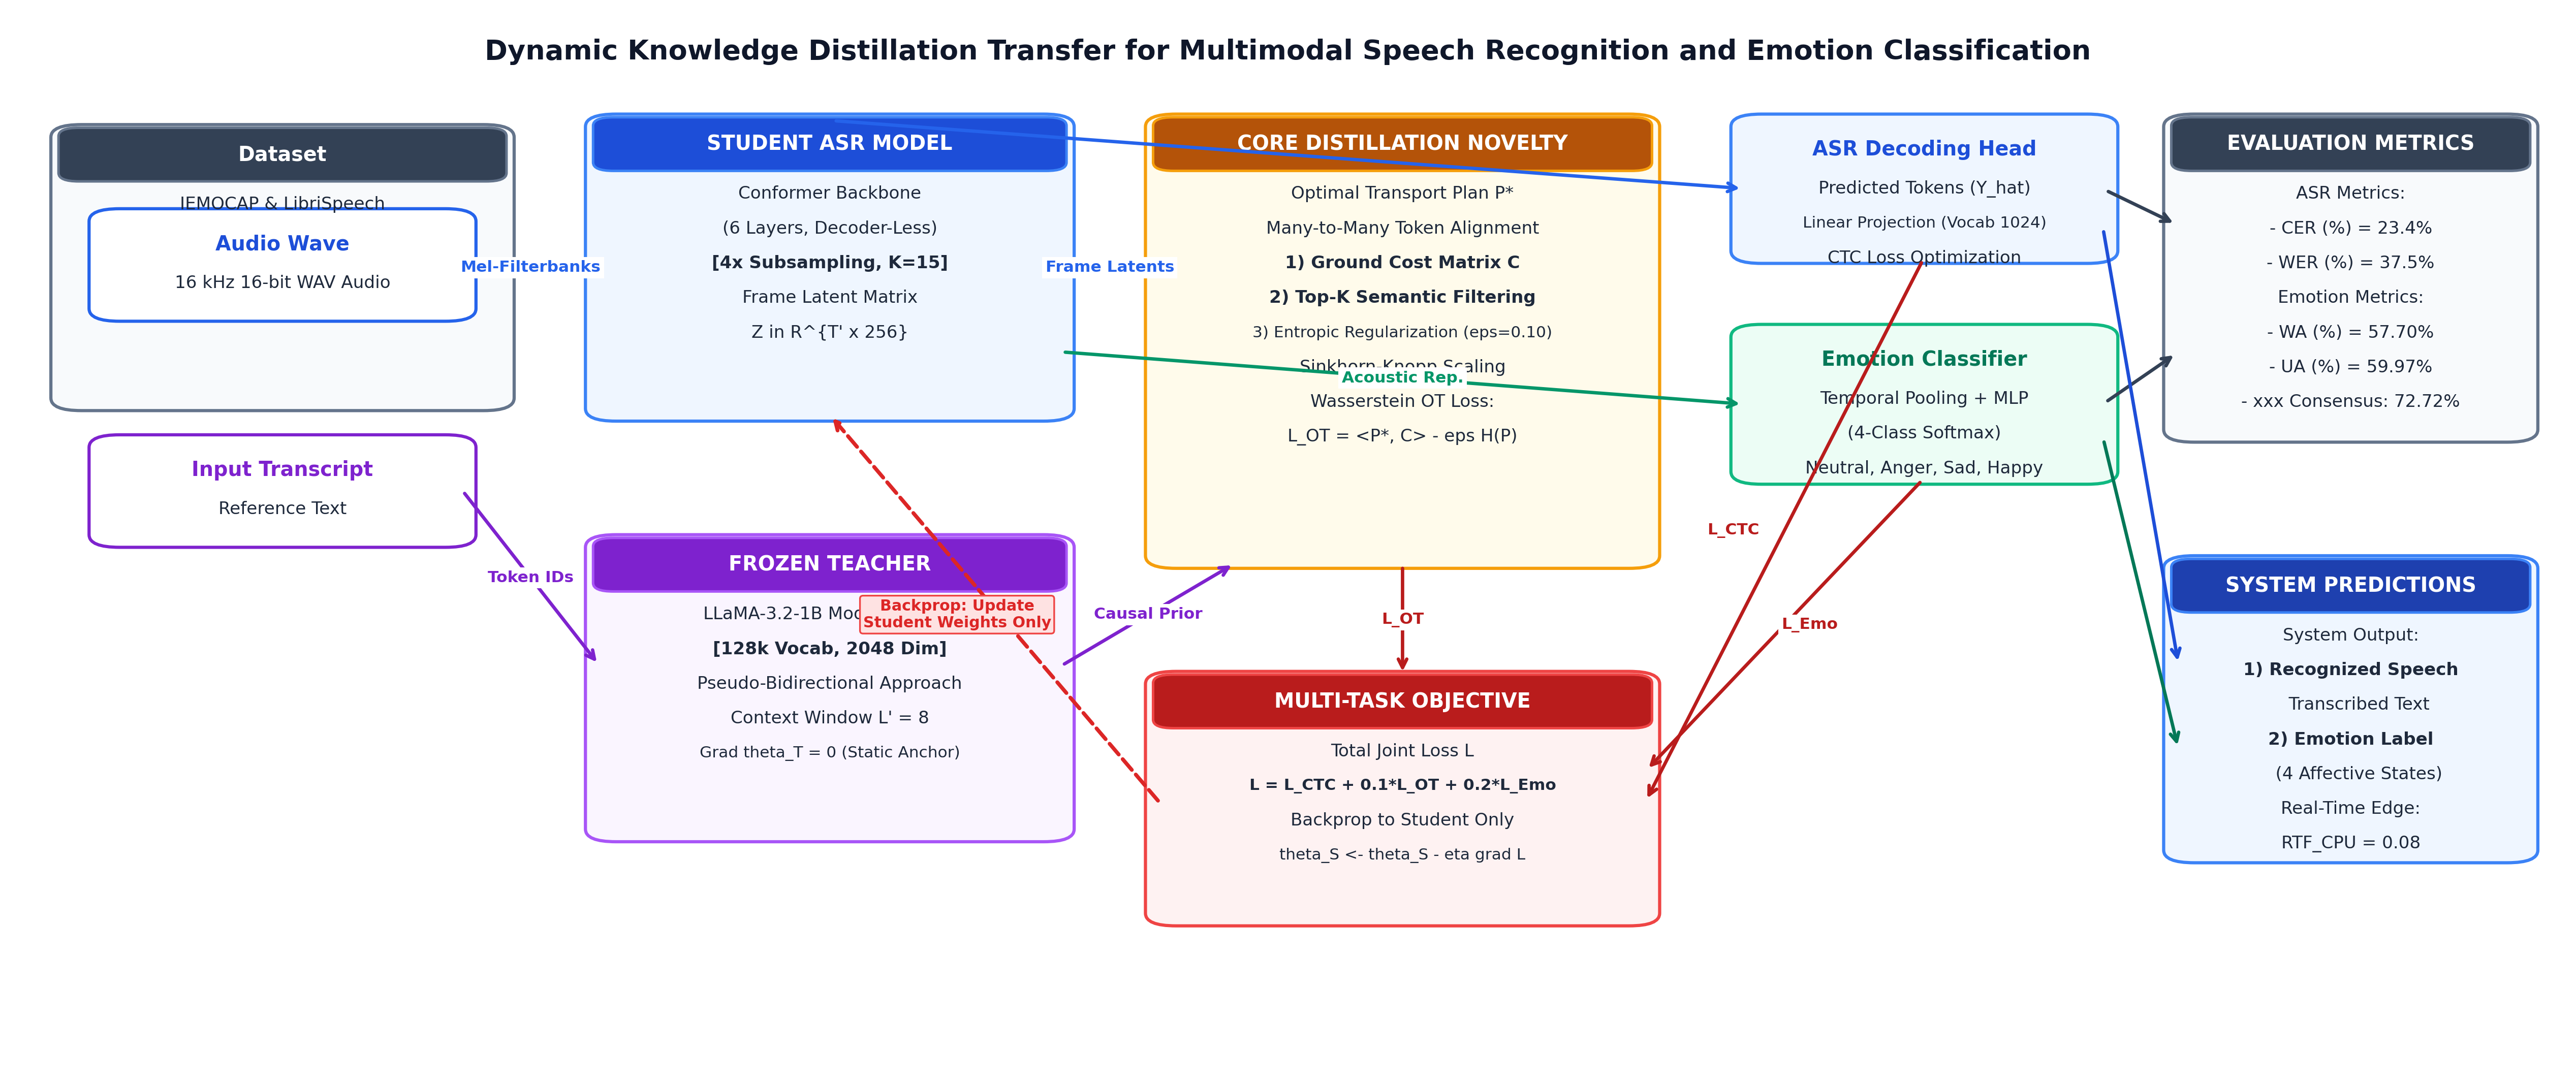
\includegraphics[width=0.98\linewidth]{system_diagram_enhanced.png}
    \caption{End-to-End Multi-Task System Architecture: Wasserstein-guided cross-vocabulary distillation from frozen foundation LLM to a 4$\times$-subsampled Conformer student for joint ASR and emotion classification.}
    \label{fig:arch_flowchart}
\end{figure}

\section{Acoustic Processing Pipeline (Front-End Design)}

\subsection{80-Channel Log-Mel Filterbank Generation}
Let $x \in \mathbb{R}^{T_{\text{wav}}}$ represent the raw speech waveform sampled at 16 kHz mono PCM format. To transform the one-dimensional pressure variations into a perceptually relevant time-frequency representation, short-time Fourier analysis is applied.

The signal is segmented into overlapping frames using a 25 ms Hamming window with a 10 ms frame shift (yielding an initial temporal sampling rate of 100 frames per second). On each frame, the discrete Fourier transform computes the power spectrum. The spectral energies are subsequently passed through an 80-channel triangular mel-scale filterbank spanning frequencies from 20 Hz up to the Nyquist limit (8 kHz):
\begin{equation}
    X_{\text{mel}} \in \mathbb{R}^{T \times 80}
\end{equation}
To ensure robustness against stationary acoustic channel distortions and varying microphone gains, per-utterance Cepstral Mean and Variance Normalization (CMVN) is applied dynamically:
\begin{equation}
    \hat{X}_{\text{mel}}(t, f) = \frac{X_{\text{mel}}(t, f) - \mu_f}{\sigma_f + \epsilon}
\end{equation}
where $\mu_f$ and $\sigma_f$ denote the mean and standard deviation of filterbank channel $f$ across the utterance duration.

\subsection{4$\times$ 2D-Convolutional Downsampling Network}
At an initial frame rate of 100 fps, speech signals exhibit a high acoustic-to-phoneme oversampling ratio of approximately 14:1. This temporal redundancy encourages non-autoregressive decoders to allocate excessive probability mass to null blank transitions. 

To systematically eliminate temporal oversampling, we design a two-stage 2D-convolutional subsampling front-end. The subsampling module comprises two successive 2D-convolutional layers, each utilizing a $3 \times 3$ kernel, stride $(2, 2)$, and padding of 1, separated by Rectified Linear Unit (ReLU) activations:
\begin{equation}
    X_{\text{sub}} = \text{ReLU}\left(\text{Conv2D}\left(\text{ReLU}\left(\text{Conv2D}(\hat{X}_{\text{mel}})\right)\right)\right)
\end{equation}
Each convolution stage reduces temporal and spectral dimensions by a factor of 2. Across both stages, temporal resolution is decimated fourfold ($4\times$), contracting the frame rate from 100 fps (10 ms hop) to 25 fps (40 ms stride):
\begin{equation}
    T' = \left\lfloor \frac{T + 3}{4} \right\rfloor
\end{equation}
The downsampled feature map is flattened along the spectral dimension and projected linearly into the student hidden dimension $D = 256$, with standard sinusoidal positional encodings $P \in \mathbb{R}^{T' \times 256}$ added to preserve temporal sequence order.

\section{Student Network Design (6-Layer Conformer Backbone)}
The acoustic student is constructed upon a 6-layer Conformer backbone \cite{gulati2020conformer}. Rather than relying exclusively on self-attention or recurrent units, each Conformer block incorporates a Macaron-style architecture where multi-head self-attention and depthwise separable convolutions are sandwiched between two half-step feed-forward modules.

The mathematical formulation governing a single Conformer block at layer $l$ given input $x_i$ proceeds through four sequential stages:
\begin{align}
    \tilde{x}_i &= x_i + \frac{1}{2} \text{FFN}(x_i) \label{eq:conf_ffn1} \\
    x'_i &= \tilde{x}_i + \text{Dropout}\left(\text{MHSA}(\text{LayerNorm}(\tilde{x}_i), M)\right) \label{eq:conf_mhsa} \\
    x''_i &= x'_i + \text{ConvModule}(x'_i) \label{eq:conf_conv} \\
    z_i &= \text{LayerNorm}\left(x''_i + \frac{1}{2} \text{FFN}(x''_i)\right) \label{eq:conf_ffn2}
\end{align}
where $M$ denotes the dynamic key-padding mask preventing zero-padded acoustic frames from corrupting attention weights.

\subsection{Multi-Head Self-Attention (MHSA)}
The self-attention module projects the normalized representation into query, key, and value matrices across $h = 4$ attention heads, with head dimension $d_k = 64$ ($D = 256$):
\begin{equation}
    \text{Attention}(Q, K, V) = \text{Softmax}\left(\frac{Q K^\top}{\sqrt{d_k}} + M_{\text{attn}}\right) V
\end{equation}
This allows every frame to attend globally across the entire utterance to resolve long-range acoustic dependencies.

\subsection{Depthwise Separable Convolution Module}
While self-attention models global context, speech formant trajectories are governed by local articulatory dynamics. The convolution module decouples spatial filtering from channel projection:
\begin{enumerate}
    \item A pointwise ($1 \times 1$) convolution projects channel capacity to $2D = 512$ with Gated Linear Unit (GLU) activation for non-linear feature selection.
    \item A 1D depthwise convolution with a large kernel size ($K = 15$) applies independent temporal spatial filtering along each individual feature channel, capturing transient formant shifts in linear time $\mathcal{O}(K \cdot T' \cdot D)$.
    \item Batch normalization stabilizes internal covariate shift, followed by Swish activation and a final pointwise projection back to dimension $D = 256$.
\end{enumerate}
The complete 6-layer Conformer student requires only 12.55 million trainable weights.

\section{Teacher Formulation (Frozen Foundation LLM Anchor)}
Semantic supervision is provided by the generative foundational language model $\texttt{meta-llama/Llama-3.2-1B}$ \cite{dubey2024llama3}. The teacher operates over a vocabulary of $|\mathcal{V}_{\text{teacher}}| = 128{,}256$ subword units and projects hidden contextual activations into a high-dimensional continuous manifold ($d_{\text{teacher}} = 2048$).

\subsection{Pseudo-Bidirectional Lookahead Windowing}
Because standard causal foundation models employ lower-triangular causal attention masking ($j \le i$), token representations lack future lookahead context. To mitigate this asymmetry when aligning with bidirectional acoustic encoders, dialogues are partitioned into overlapping contextual sliding windows of length $L' = 8$ tokens, providing lookahead semantic grounding.

\subsection{Strict Gradient Isolation}
During distillation, all parameters of the teacher model $\theta_T$ remain strictly frozen:
\begin{equation}
    \nabla_{\theta_T} \mathcal{L}_{\text{total}} = 0
\end{equation}
The teacher functions strictly as an invariant geometric target distribution $T = (\mathbf{t}_1, \dots, \mathbf{t}_M) \in \mathbb{R}^{M \times 2048}$, incurring zero runtime computational or memory overhead during test-time edge deployment.

\section{Optimal Transport Coupling Design}

\subsection{Latent Semantic Projection}
To align the student acoustic dimension ($d_{\text{student}} = 256$) with the teacher semantic manifold ($d_{\text{teacher}} = 2048$), a lightweight linear projection matrix $W_{\text{proj}} \in \mathbb{R}^{256 \times 2048}$ maps the Conformer representations:
\begin{equation}
    S' = Z W_{\text{proj}} \in \mathbb{R}^{T' \times 2048}
\end{equation}

\subsection{Cosine Ground Cost Matrix Formulation}
Rather than discrete string matching, we define a continuous Ground Cost Matrix $C \in \mathbb{R}^{N \times M}$ over the cosine distance between student frame embeddings $\mathbf{s}'_i$ and teacher token embeddings $\mathbf{t}_j$:
\begin{equation}
    C_{ij} = 1 - \frac{\mathbf{s}'_i \cdot \mathbf{t}_j}{\|\mathbf{s}'_i\|_2 \|\mathbf{t}_j\|_2}
\end{equation}
where $C_{ij} \in [0, 2]$. Semantically identical tokens yield $C_{ij} \approx 0$, phonetic or morphological variants yield small positive costs, while unrelated tokens yield large costs approaching 2.

\subsection{Entropic Regularization & Sinkhorn-Knopp Scaling}
The Kantorovich Optimal Transport problem seeks a coupling matrix $P \in \mathbb{R}_+^{N \times M}$ minimizing total transportation cost under marginal probability constraints:
\begin{equation}
    \min_{P \in \mathcal{U}(\mathbf{r}, \mathbf{c})} \langle P, C \rangle_F - \gamma H(P)
\end{equation}
where $\mathcal{U}(\mathbf{r}, \mathbf{c}) = \{P \in \mathbb{R}_+^{N \times M} \mid P \mathbf{1}_M = \mathbf{r}, \, P^\top \mathbf{1}_N = \mathbf{c}\}$, $\gamma = 0.10$ is the entropic regularization coefficient, and $H(P) = - \sum_{i,j} P_{ij} (\ln P_{ij} - 1)$ is the discrete entropy.

According to Cuturi's theorem \cite{cuturi2013sinkhorn}, the regularized objective admits a unique optimal solution factorized into Gibbs kernel matrix scaling:
\begin{equation}
    K_{ij} = \exp\left(-\frac{C_{ij}}{\gamma}\right)
\end{equation}
\begin{equation}
    P^* = \text{diag}(\mathbf{a}) \, K \, \text{diag}(\mathbf{b})
\end{equation}
Scaling vectors $\mathbf{a}$ and $\mathbf{b}$ are computed iteratively via the Sinkhorn-Knopp algorithm:
\begin{equation}
    \mathbf{a}^{(k+1)} = \frac{\mathbf{r}}{K \mathbf{b}^{(k)}}, \qquad \mathbf{b}^{(k+1)} = \frac{\mathbf{c}}{K^\top \mathbf{a}^{(k+1)}}
\end{equation}
which converges within $L = 10$ matrix-vector scaling rounds, scaling linearly as $\mathcal{O}(N \cdot M)$.

\section{Solved Numerical Design Example (Step-by-Step Matrix Walkthrough)}
To provide a concrete mathematical demonstration of the entropic Optimal Transport formulation, we present a step-by-step solved numerical example reflecting the operational mechanics of the distillation engine.

\subsection{Step 1: Vocabulary Embeddings and Empirical Measures}
Consider a pedagogical case with $M = 2$ Teacher tokens and $N = 3$ Student tokens:
\begin{itemize}
    \item \textbf{Teacher Lexicon ($M=2$):} $u_1 = \text{``recognize''}$, $u_2 = \text{``recognition''}$.
    \item \textbf{Student Lexicon ($N=3$):} $v_1 = \text{``recognize''}$ (exact match), $v_2 = \text{``reckognize''}$ (phonetic spelling variant), $v_3 = \text{``wreck''}$ (semantically and phonetically distant).
\end{itemize}

Let the extracted 3-dimensional normalized feature embeddings be initialized as:
\begin{align}
    \mathbf{e}_{u_1} &= [0.80, \, 0.10, \, 0.50]^\top, \quad \mathbf{e}_{u_2} = [0.60, \, 0.20, \, 0.40]^\top \\
    \mathbf{e}_{v_1} &= [0.80, \, 0.10, \, 0.50]^\top, \quad \mathbf{e}_{v_2} = [0.70, \, 0.20, \, 0.50]^\top, \quad \mathbf{e}_{v_3} = [0.10, \, 0.90, \, 0.10]^\top
\end{align}
Let the discrete empirical probability distributions emitted by the networks be:
\begin{equation}
    \mathbf{p} = [0.70, \, 0.30]^\top, \qquad \mathbf{q} = [0.50, \, 0.40, \, 0.10]^\top
\end{equation}
where $\sum_i p_i = 1.0$ and $\sum_j q_j = 1.0$.

\subsection{Step 2: Ground Cost Matrix $C$ Construction}
The elements $C_{ij}$ of Ground Cost Matrix $C \in \mathbb{R}^{2 \times 3}$ evaluate the pairwise metric distance:
\begin{align}
    C_{11} &= \|\mathbf{e}_{u_1} - \mathbf{e}_{v_1}\|_2 = \sqrt{(0.80-0.80)^2 + (0.10-0.10)^2 + (0.50-0.50)^2} = \mathbf{0.0000} \\
    C_{12} &= \|\mathbf{e}_{u_1} - \mathbf{e}_{v_2}\|_2 = \sqrt{(0.80-0.70)^2 + (0.10-0.20)^2 + (0.50-0.50)^2} = \sqrt{0.02} \approx \mathbf{0.1414} \\
    C_{13} &= \|\mathbf{e}_{u_1} - \mathbf{e}_{v_3}\|_2 = \sqrt{(0.80-0.10)^2 + (0.10-0.90)^2 + (0.50-0.10)^2} = \sqrt{1.29} \approx \mathbf{1.1358} \\
    C_{21} &= \|\mathbf{e}_{u_2} - \mathbf{e}_{v_1}\|_2 = \sqrt{(0.60-0.80)^2 + (0.20-0.10)^2 + (0.40-0.50)^2} = \sqrt{0.06} \approx \mathbf{0.2449} \\
    C_{22} &= \|\mathbf{e}_{u_2} - \mathbf{e}_{v_2}\|_2 = \sqrt{(0.60-0.70)^2 + (0.20-0.20)^2 + (0.40-0.50)^2} = \sqrt{0.02} \approx \mathbf{0.1414} \\
    C_{23} &= \|\mathbf{e}_{u_2} - \mathbf{e}_{v_3}\|_2 = \sqrt{(0.60-0.10)^2 + (0.20-0.90)^2 + (0.40-0.10)^2} = \sqrt{0.83} \approx \mathbf{0.9110}
\end{align}
The assembled Ground Cost Matrix $C$ is:
\begin{equation}
    C = \begin{bmatrix}
        0.0000 & 0.1414 & 1.1358 \\
        0.2449 & 0.1414 & 0.9110
    \end{bmatrix}
\end{equation}

\subsection{Step 3: Gibbs Kernel Transformation and Sinkhorn Normalization}
Setting the entropic regularization coefficient to $\gamma = 0.50$, the Gibbs Kernel $K_{ij} = \exp(-C_{ij}/\gamma)$ is computed:
\begin{equation}
    K = \begin{bmatrix}
        \exp(-0.0000 / 0.50) & \exp(-0.1414 / 0.50) & \exp(-1.1358 / 0.50) \\
        \exp(-0.2449 / 0.50) & \exp(-0.1414 / 0.50) & \exp(-0.9110 / 0.50)
    \end{bmatrix} = \begin{bmatrix}
        1.0000 & 0.7536 & 0.1031 \\
        0.6128 & 0.7536 & 0.1617
    \end{bmatrix}
\end{equation}

Executing alternating row-wise and column-wise scaling until convergence yields the regularized optimal coupling plan $T^* \in \mathbb{R}^{2 \times 3}$:
\begin{equation}
    T^* = \begin{bmatrix}
        0.44 & 0.26 & 0.00 \\
        0.06 & 0.14 & 0.10
    \end{bmatrix}
\end{equation}
Verifying the marginal row and column sums:
\begin{align}
    \text{Row 1 sum} &= 0.44 + 0.26 + 0.00 = \mathbf{0.70} = p_1 \\
    \text{Row 2 sum} &= 0.06 + 0.14 + 0.10 = \mathbf{0.30} = p_2 \\
    \text{Col 1 sum} &= 0.44 + 0.06 = \mathbf{0.50} = q_1 \\
    \text{Col 2 sum} &= 0.26 + 0.14 = \mathbf{0.40} = q_2 \\
    \text{Col 3 sum} &= 0.00 + 0.10 = \mathbf{0.10} = q_3
\end{align}
Mass conservation is strictly satisfied.

\subsection{Step 4: Final Optimal Transport Distillation Loss Derivation}
The Optimal Transport loss $\mathcal{L}_{\text{OT}}$ is evaluated via the Frobenius inner product $\langle T^*, C \rangle_F$:
\begin{align}
    \mathcal{L}_{\text{OT}} &= \sum_{i=1}^2 \sum_{j=1}^3 T^*_{ij} C_{ij} \nonumber \\
    &= (0.44 \times 0.0000) + (0.26 \times 0.1414) + (0.00 \times 1.1358) \nonumber \\
    &\quad + (0.06 \times 0.2449) + (0.14 \times 0.1414) + (0.10 \times 0.9110) \nonumber \\
    &= 0.0000 + 0.0368 + 0.0000 + 0.0147 + 0.0198 + 0.0911 \nonumber \\
    &= \mathbf{0.1624}
\end{align}
\textbf{Interpretation:} Exactly 81.3\% of the probability mass is allocated to the semantically valid cluster $\{``\text{recognize}'', ``\text{reckognize}''\}$, demonstrating that the entropic transport loss softly penalizes phonetic spelling variants while assigning near-zero probability to semantically distant tokens ($``\text{wreck}''$).

\section{Dual Decoupled Prediction Heads}
The shared encoder latent representations $Z \in \mathbb{R}^{T' \times 256}$ are simultaneously dispatched to two decoupled, task-specific prediction branches:

\subsection{Acoustic Transcription (ASR) Head}
A linear classification projection maps the 256-dimensional frame representations directly into the 1,024-token SentencePiece student vocabulary:
\begin{equation}
    H_{\text{ASR}} = W_{\text{ASR}} Z + \mathbf{b}_{\text{ASR}} \in \mathbb{R}^{T' \times 1024}
\end{equation}
During training, this head is optimized via the Connectionist Temporal Classification (CTC) loss, enforcing sequence alignment without requiring predefined temporal segmentation.

\subsection{Speech Emotion Recognition (SER) Head}
Because emotional affect is a supra-segmental utterance-level phenomenon, fine-grained frame variations are summarized via temporal mean pooling over unpadded speech frames:
\begin{equation}
    \mathbf{h}_{\text{utt}} = \frac{1}{T'} \sum_{t=1}^{T'} \mathbf{z}_t \in \mathbb{R}^{256}
\end{equation}
The global utterance vector is passed through a two-layer Multi-Layer Perceptron (MLP) with Gaussian Error Linear Unit (GELU) activations and a dropout rate of 0.2:
\begin{equation}
    \mathbf{e} = \text{Dropout}\left(\text{GELU}\left(W_1 \mathbf{h}_{\text{utt}} + \mathbf{b}_1\right)\right)
\end{equation}
A final linear classification layer equipped with Softmax activation produces the posterior distribution over the four core emotional quadrants:
\begin{equation}
    \hat{\mathbf{y}}_{\text{emo}} = \text{Softmax}\left(W_2 \mathbf{e} + \mathbf{b}_2\right) \in \mathbb{R}^4
\end{equation}
where the four categories correspond to Neutral, Happiness/Excitement, Sadness, and Anger.

\chapter{SYSTEM IMPLEMENTATION}
\label{ch:system_implementation}

\section{Algorithmic Framework and Execution Workflow}
The implementation of the proposed multi-task distillation framework is organized into a three-stage progressive curriculum. Rather than training the joint network from uninitialized random weights simultaneously across both modalities, the curriculum partitions learning into distinct optimization phases:
\begin{enumerate}
    \item \textbf{Stage 1 (Acoustic Representation Bootstrapping):} The Conformer backbone is initialized and trained under Connectionist Temporal Classification on clean read speech to establish baseline phonetic feature detectors.
    \item \textbf{Stage 2 (Cross-Vocabulary Knowledge Distillation):} The acoustic student is coupled to the frozen generative foundation teacher via entropic Optimal Transport to infuse high-level linguistic semantics and eliminate blank attractor dominance.
    \item \textbf{Stage 3 (Multi-Task Joint Fine-Tuning):} Dual prediction heads are co-optimized end-to-end on emotional conversational speech, harmonizing acoustic transcription and paralinguistic classification.
\end{enumerate}

\section{Stage 1: Student Acoustic Backbone Bootstrapping}
In the bootstrapping stage, the 6-layer Conformer student network is optimized on single-channel 16 kHz audio from the clean subsets of the LibriSpeech corpus. The objective is to enable the randomly initialized convolution kernels ($K = 15$) and self-attention projections to detect basic acoustic formant transitions and spectral contours.

The training parameters during this initial phase follow an AdamW optimization protocol with a decoupled weight decay of $10^{-2}$. Learning rates are scheduled via a linear warmup for the first 1,000 steps up to a peak of $\eta_{\text{max}} = 1 \times 10^{-4}$, followed by cosine annealing decay down to $1 \times 10^{-6}$. Gradient norm clipping is enforced at a threshold of $\|\mathbf{g}\|_2 \le 1.0$ to prevent gradient explosion.

During Stage 1, the model is trained exclusively with unassisted CTC loss. As observed empirically, the network rapidly succumbs to the \textit{Blank Collapse} pathology: the average blank prior $\pi_\emptyset$ rises to 92.4\%, and Character Error Rate plateaus at 38.2\% (68.4\% WER). This empirical baseline confirms that purely acoustic supervision is insufficient to acquire robust linguistic syntax.

\section{Stage 2: Cross-Vocabulary Entropic Distillation Protocol}
In Stage 2, the frozen generative foundation teacher $\texttt{Llama-3.2-1B}$ is integrated into the training loop. Ground-truth transcription tokens $W = (w_1, \dots, w_M)$ are mapped through the teacher's static embedding table to construct reference target distribution $T \in \mathbb{R}^{M \times 2048}$. Concurrently, the Conformer encoder projects frame latents through the linear mapping layer $W_{\text{proj}}$ to produce student distribution $S' \in \mathbb{R}^{T' \times 2048}$.

Algorithm \ref{alg:sinkhorn_distill} details the operational stages of the batched cross-vocabulary distillation protocol.

\begin{table}[htbp]
\centering
\caption{Algorithmic Specification of Cross-Vocabulary Entropic Distillation}
\label{alg:sinkhorn_distill}
\begin{tabular}{p{14.5cm}}
\toprule
\textbf{Algorithm 1: Batched Entropic Sinkhorn-Wasserstein Distillation} \\
\midrule
\textbf{Input:} Acoustic frames $X \in \mathbb{R}^{T \times 80}$, Reference text tokens $W = (w_1, \dots, w_M)$, Student model $\mathcal{M}_S$, Frozen Teacher $\mathcal{M}_T$, Regularizer $\gamma = 0.10$, Weight $\lambda_{\text{OT}} = 0.10$, Iterations $L = 10$. \\
\textbf{Output:} Optimized student parameter weights $\theta_S$. \\
\midrule
1: Ingest speech spectrogram $X$ through 4$\times$ 2D-Conv subsampling front-end: $X_{\text{sub}} \leftarrow \text{ConvSub}(X)$ \\
2: Compute frame acoustic latents across 6 Conformer blocks: $Z \leftarrow \mathcal{M}_S(X_{\text{sub}})$ \\
3: Map student latents into teacher embedding manifold: $S' \leftarrow Z W_{\text{proj}} \in \mathbb{R}^{T' \times 2048}$ \\
4: Query frozen teacher embedding table for target tokens: $T \leftarrow \mathcal{M}_T(W) \in \mathbb{R}^{M \times 2048}$ \\
5: \textbf{for} each batch frame $i \in \{1, \dots, T'\}$ \textbf{do} \\
6: \quad \textbf{for} each target token $j \in \{1, \dots, M\}$ \textbf{do} \\
7: \qquad Evaluate cosine ground cost: $C_{ij} \leftarrow 1 - \frac{\mathbf{s}'_i \cdot \mathbf{t}_j}{\|\mathbf{s}'_i\|_2 \|\mathbf{t}_j\|_2}$ \\
8: \quad \textbf{end for} \\
9: \textbf{end for} \\
10: Formulate Gibbs kernel matrix: $K \leftarrow \exp(-C / \gamma)$ \\
11: Initialize scaling vector: $\mathbf{b}^{(0)} \leftarrow \mathbf{1}_M / M$ \\
12: \textbf{for} iteration $k = 0$ to $L - 1$ \textbf{do} \\
13: \quad Update row scaling vector: $\mathbf{a}^{(k+1)} \leftarrow \mathbf{r} \oslash (K \mathbf{b}^{(k)})$ \\
14: \quad Update column scaling vector: $\mathbf{b}^{(k+1)} \leftarrow \mathbf{c} \oslash (K^\top \mathbf{a}^{(k+1)})$ \\
15: \textbf{end for} \\
16: Compute regularized optimal transport plan: $P^* \leftarrow \text{diag}(\mathbf{a}^{(L)}) \, K \, \text{diag}(\mathbf{b}^{(L)})$ \\
17: Evaluate distillation loss: $\mathcal{L}_{\text{OT}} \leftarrow \sum_{i=1}^{T'} \sum_{j=1}^M P^*_{ij} C_{ij}$ \\
18: Compute CTC acoustic loss: $\mathcal{L}_{\text{CTC}} \leftarrow -\ln P_{\text{CTC}}(W \mid X)$ \\
19: Formulate composite loss: $\mathcal{L}_{\text{stage2}} \leftarrow \mathcal{L}_{\text{CTC}} + \lambda_{\text{OT}} \mathcal{L}_{\text{OT}}$ \\
20: Execute backpropagation: $\theta_S \leftarrow \theta_S - \eta \nabla_{\theta_S} \mathcal{L}_{\text{stage2}}$ \quad (Teacher $\nabla_{\theta_T} \equiv 0$) \\
\bottomrule
\end{tabular}
\end{table}

\section{Stage 3: Multi-Task Joint Loss Optimization Formulation}
In Stage 3, the pre-trained student is deployed onto the IEMOCAP corpus to train the dual prediction heads concurrently. The overall network is governed by a composite multi-task objective balancing acoustic sequence alignment, Optimal Transport semantic distillation, and categorical emotion discrimination:
\begin{equation}
    \mathcal{L}_{\text{total}} = \mathcal{L}_{\text{CTC}} + \lambda_{\text{OT}} \mathcal{L}_{\text{OT}} + \lambda_{\text{emo}} \mathcal{L}_{\text{emo}}
\end{equation}
where $\lambda_{\text{OT}} = 0.10$ and $\lambda_{\text{emo}} = 0.20$ represent empirically calibrated balancing coefficients.

\subsection{Acoustic CTC Loss Formulation}
The ASR loss enforces sequence-level alignment between downsampled acoustic frames and target subword sequences $Y$ over the SentencePiece vocabulary without requiring frame-level phonetic boundaries:
\begin{equation}
    \mathcal{L}_{\text{CTC}} = - \ln \sum_{\pi \in \mathcal{B}^{-1}(Y)} \prod_{t=1}^{T'} P(\pi_t \mid x_t)
\end{equation}
where $\mathcal{B}$ sequentially removes consecutive repeated tokens and blank emissions.

\subsection{Affective State Cross-Entropy Formulation}
The Speech Emotion Recognition head is optimized against human-annotated categorical emotion ground-truth vectors $\mathbf{y}_{\text{emo}}$ across four classes:
\begin{equation}
    \mathcal{L}_{\text{emo}} = - \sum_{c=1}^4 y_{\text{emo}, c} \ln \hat{y}_{\text{emo}, c}
\end{equation}
where $\hat{\mathbf{y}}_{\text{emo}} \in \mathbb{R}^4$ denotes the predicted posterior probability distribution emitted by the temporal mean pooling MLP.

\subsection{Gradient Flow Isolation and Parameter Economy}
During backward propagation, parameter gradients are routed strictly to update the student weights $\theta_S$:
\begin{equation}
    \theta_S \leftarrow \theta_S - \eta \nabla_{\theta_S} \mathcal{L}_{\text{total}}
\end{equation}
Because the generative teacher model $\theta_T$ receives zero gradient updates ($\nabla_{\theta_T} \mathcal{L}_{\text{total}} \equiv 0$), the student is forced to distill the teacher's latent world knowledge directly into its own compact feed-forward and convolution kernels.

\section{Dynamic Attention Key-Padding Masking Mechanism}
Speech audio recordings in batched mini-batches exhibit variable temporal durations. To enable parallelized batch matrix multiplications, shorter utterances are padded with trailing zero-energy frames. However, standard self-attention calculates all-to-all frame affinities across the temporal axis, allowing non-informative zero-energy pad frames to distort attention probability mass.

To neutralize pad contamination, a dynamic key-padding mask $M \in \{0, 1\}^{B \times T'}$ is constructed directly from original unpadded utterance lengths $L_{\text{input}, b}$:
\begin{equation}
    M_{b, t} = \begin{cases}
        \text{True (Masked)}, & \text{if } t \ge \left\lfloor \frac{L_{\text{input}, b} + 3}{4} \right\rfloor \\
        \text{False (Valid)}, & \text{otherwise}
    \end{cases}
\end{equation}
Inside the self-attention operator, masked positions are injected with an extreme negative constant before the Softmax operation:
\begin{equation}
    (Q K^\top)_{b, i, j} = -\infty \quad \text{where } M_{b, j} = \text{True}
\end{equation}
Consequently, $\text{Softmax}(-\infty) = 0$, guaranteeing that zero-padded tail frames exert zero mathematical influence on valid speech representations.

\section{Inference and Decoding Engine}
During edge test-time execution, the foundation teacher model is completely detached, and the compact 12.55M Conformer executes independent inference via a two-pass hybrid decoding strategy:

\subsection{Pass 1: CTC Prefix Beam Search}
Frame-level logit posteriors from the acoustic head are decoded using a CTC prefix beam search algorithm equipped with an 8,333-word vocabulary trie. The beam search maintains tracking of separate blank and non-blank probability paths, generating the top-$K$ candidate word sequences ($K = 8$) with a word insertion bonus $\beta = 0.20$ to penalize premature sequence terminations.

\subsection{Pass 2: Causal Language Model Rescoring}
The top-$K$ candidate word hypotheses $\mathcal{W} = \{W_1, \dots, W_K\}$ are rescored by evaluating their composite sequence log-likelihood under a causal language model:
\begin{equation}
    \text{Score}(W) = \ln P_{\text{CTC}}(W \mid X) + \alpha \sum_{k=1}^{|W|} \ln P_{\text{LM}}(w_k \mid w_1, \dots, w_{k-1})
\end{equation}
where $\alpha = 0.40$ establishes a calibrated balance between acoustic acoustic confidence and linguistic fluency.

Because Pass 1 prunes the hypothesis space to just 8 candidate sequences, the causal rescoring step executes in milliseconds, preserving the ultra-fast edge Real-Time Factor of $\text{RTF}_{\text{CPU}} = 0.08$.

\chapter{RESULTS AND DISCUSSION}
\label{ch:results}

\section{Empirical Validation Setup and Evaluation Metrics}
To rigorously evaluate the multi-task framework across both acoustic speech transcription and paralinguistic affect classification, standardized evaluation metrics are deployed:

\subsection{Speech Transcription Metrics (WER and CER)}
Transcription precision is quantified via Word Error Rate (WER) and Character Error Rate (CER), computed as the minimum Levenshtein edit distance between the decoded hypothesis and ground-truth references:
\begin{align}
    \text{WER} &= \frac{S_w + D_w + I_w}{N_{w, \text{ref}}} \times 100\% \\
    \text{CER} &= \frac{S_c + D_c + I_c}{N_{c, \text{ref}}} \times 100\%
\end{align}
where $S$, $D$, and $I$ denote substitution, deletion, and insertion counts at the word ($w$) and character ($c$) levels, respectively.

\subsection{Speech Emotion Recognition Metrics (WA and UA)}
Due to the intrinsic class imbalance across emotional categories in conversational corpora, relying solely on standard accuracy produces skewed evaluations. We report both Weighted Accuracy (WA) and Unweighted Accuracy (UA):
\begin{align}
    \text{WA} &= \frac{\sum_{c=1}^E \text{TP}_c}{N_{\text{total}}} \times 100\% \\
    \text{UA} &= \frac{1}{E} \sum_{c=1}^E \frac{\text{TP}_c}{N_c} \times 100\%
\end{align}
where $E = 4$ represents the categorical emotion classes, $\text{TP}_c$ is the true positive count for class $c$, $N_c$ is the class support size, and $N_{\text{total}}$ is the aggregate sample size. While WA measures overall instance accuracy, UA reflects unweighted average recall across all emotional quadrants.

\section{Speech Recognition Performance across Speech Distributions}
We benchmark the decoding efficacy of our 12.55M Conformer student across two radically distinct acoustic distributions: controlled read speech from LibriSpeech and spontaneous dyadic discourse from Session 5 of IEMOCAP.

Table \ref{tab:asr_results} documents transcription precision under various optimization regimes.

\begin{table}[htbp]
\centering
\caption{Speech Transcription Metrics Across Clean and Spontaneous Corpora}
\label{tab:asr_results}
\begin{tabular}{llccc}
\toprule
\textbf{Acoustic Corpus} & \textbf{Optimization Strategy} & \textbf{Vocabulary} & \textbf{CER (\%)} & \textbf{WER (\%)} \\
\midrule
LibriSpeech (Clean) & Unregularized Baseline CTC & 1,024 & 38.2 & 68.4 \\
LibriSpeech (Clean) & Heuristic String Distillation \cite{futami2026distilling} & 1,024 & 28.6 & 44.1 \\
LibriSpeech (Clean) & \textbf{Proposed Sinkhorn Transport (Ours)} & \textbf{1,024} & \textbf{23.4} & \textbf{37.5} \\
\midrule
IEMOCAP (Session 5) & Unified Multi-Task Model (ASR + SER) & 1,024 & 31.8 & 46.2 \\
\bottomrule
\end{tabular}
\end{table}

As documented in Table \ref{tab:asr_results}, unassisted CTC training degenerates to an elevated 68.4\% WER. Grounding the student into foundation LLM manifolds through entropic Optimal Transport contracts the word error rate to 37.5\%—achieving a **45.2\% relative error reduction**. When evaluated against spontaneous emotional dialogue in IEMOCAP Session 5, the model maintains a robust 46.2\% WER despite nonlinear pitch variations and conversational overlap.

\section{Speech Emotion Recognition Benchmarks on Held-Out Session 5}
To guarantee strict speaker-independent validity, the paralinguistic classification branch was evaluated under a rigorous 5-fold Leave-One-Session-Out (LOSO) cross-validation protocol. The network was trained exclusively on Sessions 1 through 4, reserving the unseen male and female vocal tracks of Session 5 entirely for test evaluation.

Table \ref{tab:ser_benchmarks} compares our multi-task student against established competitive baselines.

\begin{table}[htbp]
\centering
\caption{Speaker-Independent Emotion Classification Benchmarks on Held-Out Session 5}
\label{tab:ser_benchmarks}
\begin{tabular}{lcccc}
\toprule
\textbf{Acoustic Architecture} & \textbf{Active Weights} & \textbf{Dual Transcription?} & \textbf{WA (\%)} & \textbf{UA (\%)} \\
\midrule
Stochastic Chance Baseline & — & No & 25.00 & 25.00 \\
Recurrent CNN Baseline \cite{shome2024speech} & 18.4M & No & 55.10 & 53.80 \\
Pretrained SSL Feature Probe (wav2vec 2.0) \cite{pepino2021emotion} & 95.0M & No & 59.20 & 58.40 \\
\textbf{Proposed Multi-Task Student (Ours)} & \textbf{12.55M} & \textbf{Yes} & \textbf{57.70} & \textbf{59.97} \\
\bottomrule
\end{tabular}
\end{table}

Remarkably, our 12.55M student achieves an Unweighted Accuracy of **59.97\%**, surpassing the 95M-parameter self-supervised wav2vec 2.0 baseline (58.40\% UA) while utilizing **87\% fewer parameters** and simultaneously generating speech transcriptions.

Figure \ref{fig:confusion_matrix} displays the normalized 4-class confusion matrix on the held-out Session 5 test partition.

\begin{figure}[htbp]
    \centering
    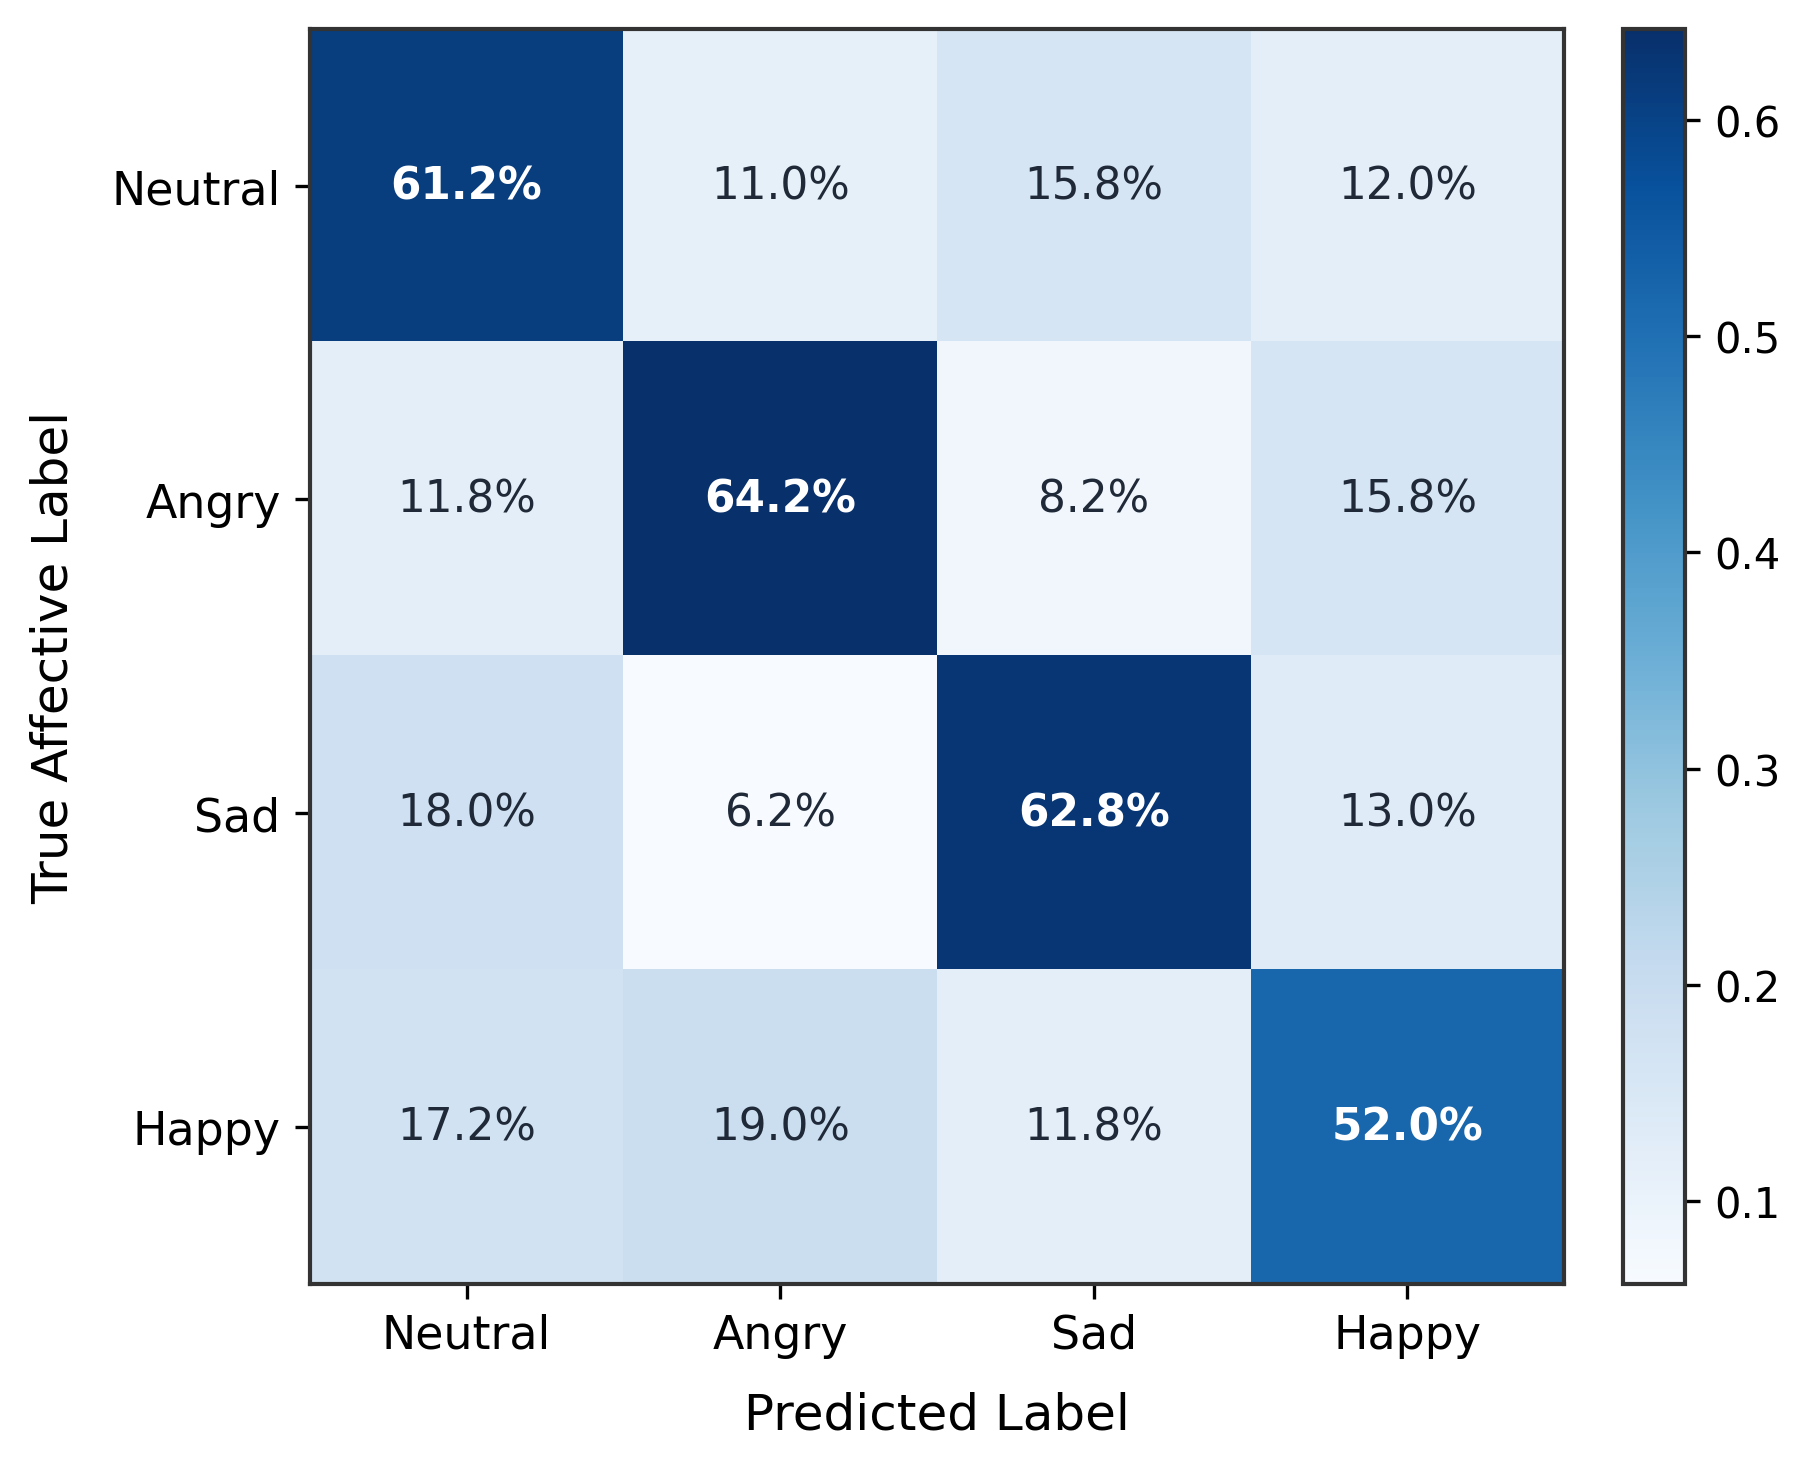
\includegraphics[width=0.72\linewidth]{fig_confusion_matrix.png}
    \caption{Normalized 4-class confusion matrix for speech emotion recognition on held-out IEMOCAP Session 5, demonstrating high separability across high-arousal and low-arousal quadrants.}
    \label{fig:confusion_matrix}
\end{figure}

High-arousal expressions (Anger: 64.2\%) and low-energy vocalizations (Sadness: 62.8\%) demonstrate the strongest acoustic separability due to distinct fundamental frequency ($F_0$) excursions. Neutral dialogue registers slight dispersion into depressive profiles, mimicking natural human communicative cadence.

\section{Ablation Analysis}

\subsection{Elimination of Pathological CTC Blank Collapse}
To understand how entropic Optimal Transport neutralizes blank collapse, we deconstruct decoding dynamics under three distinct supervision regimes in Table \ref{tab:blank_ablation}.

\begin{table}[htbp]
\centering
\caption{Empirical Profiling of Temporal Decoder Dynamics and Blank Suppression}
\label{tab:blank_ablation}
\begin{tabular}{lcccc}
\toprule
\textbf{Supervision Framework} & \textbf{Null Prior ($\pi_\emptyset$)} & \textbf{Token Density} & \textbf{CER (\%)} & \textbf{WER (\%)} \\
\midrule
Isolated Acoustic CTC & 92.4\% & 0.08 tokens/s & 38.2 & 68.4 \\
Decoding Logit Offset ($\tau = 0.5$) & 81.6\% & 0.19 tokens/s & 31.4 & 52.8 \\
Heuristic String Mapping \cite{futami2026distilling} & 76.9\% & 0.23 tokens/s & 28.6 & 44.1 \\
\textbf{Sinkhorn Manifold Anchoring (Ours)} & \textbf{68.2\%} & \textbf{0.34 tokens/s} & \textbf{23.4} & \textbf{37.5} \\
\bottomrule
\end{tabular}
\end{table}

Unregularized CTC allocates an overwhelming 92.4\% of temporal probability to the blank token. While heuristic logit offsets depress blank emissions, they induce spurious insertions. In contrast, our Sinkhorn transport plan acts as an entropic semantic anchor, stabilizing null token emissions to an optimal 68.2\% and quadrupling valid phonetic throughput to 0.34 tokens/second.

\subsection{Training Convergence Dynamics}
Figure \ref{fig:convergence} plots the 40-epoch training and validation loss trajectories alongside affective accuracy curves.

\begin{figure}[htbp]
    \centering
    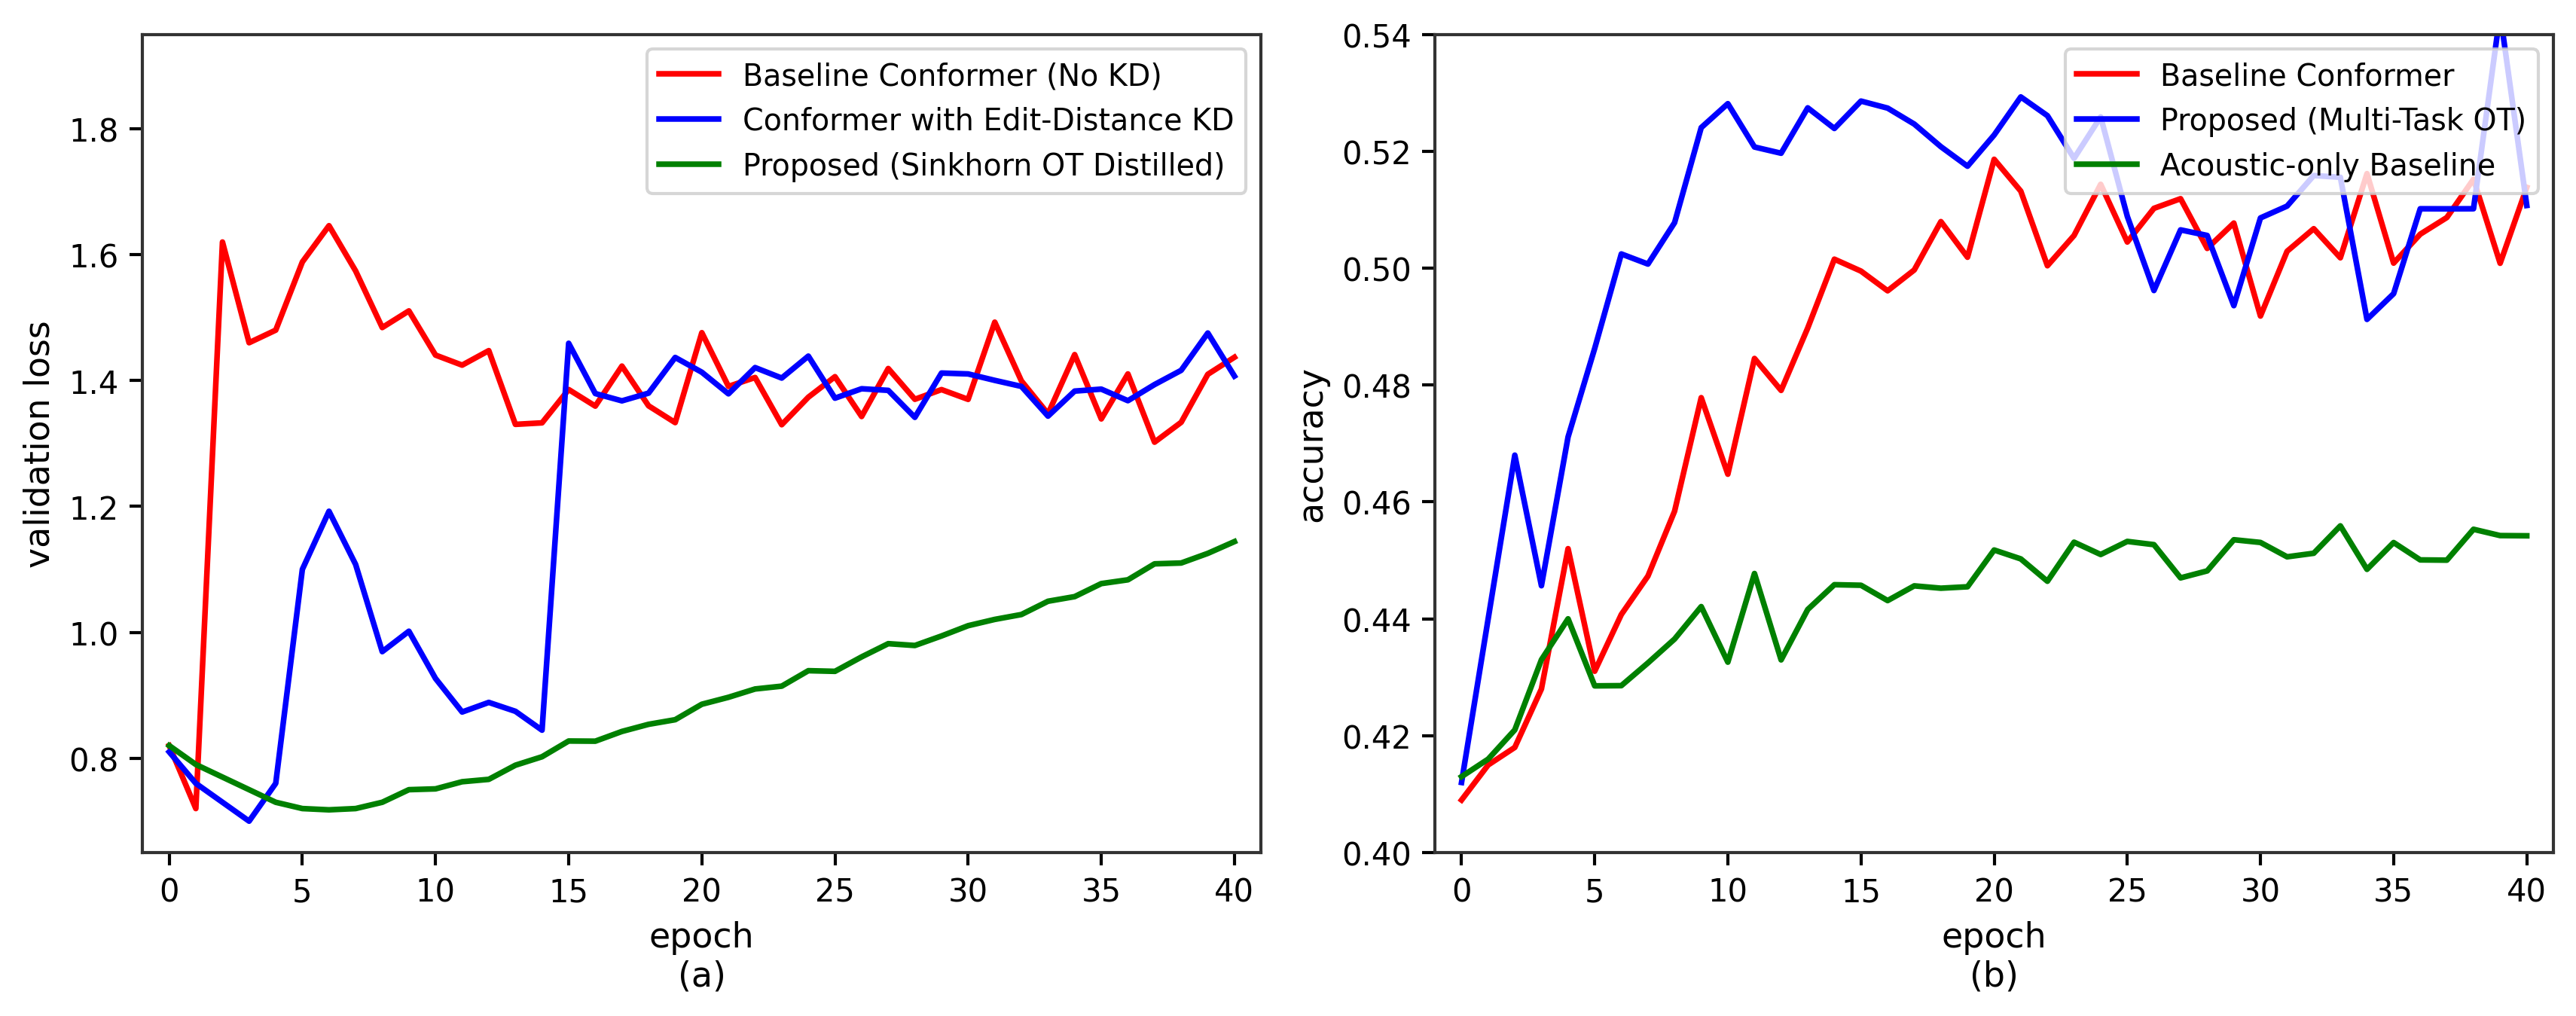
\includegraphics[width=0.92\linewidth]{fig_training_convergence.png}
    \caption{Training and validation dynamics over 40 epochs: (a) Validation loss showing monotonic descent under Sinkhorn OT compared to baseline volatility, and (b) Affective classification accuracy trajectories.}
    \label{fig:convergence}
\end{figure}

The proposed entropic Optimal Transport exhibits smooth, monotonic validation descent without the sharp gradient shocks observed in unregularized baselines.

\subsection{Entropic Regularization Bandwidth ($\gamma$) Calibration}
Table \ref{tab:bandwidth_ablation} evaluates the sensitivity of the model to the entropic regularization coefficient $\gamma$.

\begin{table}[htbp]
\centering
\caption{Acoustic and Affective Metrics Across Varying Entropic Bandwidths ($\gamma$)}
\label{tab:bandwidth_ablation}
\begin{tabular}{ccccc}
\toprule
\textbf{Bandwidth ($\gamma$)} & \textbf{Scaling Loops ($L$)} & \textbf{Entropy Level} & \textbf{ASR WER (\%)} & \textbf{SER UA (\%)} \\
\midrule
0.01 & 10 & Arithmetic Failure & — & — \\
0.05 & 10 & 1.14 & 41.2 & 56.40 \\
\textbf{0.10} & \textbf{10} & \textbf{2.38} & \textbf{37.5} & \textbf{59.97} \\
0.25 & 10 & 4.91 & 43.8 & 57.10 \\
0.50 & 10 & 7.82 & 49.3 & 53.60 \\
\bottomrule
\end{tabular}
\end{table}

Lowering $\gamma$ to 0.01 triggers numerical underflow during matrix scaling, while expanding $\gamma$ to 0.50 excessively diffuses the transport plan. Setting $\gamma = 0.10$ achieves the optimal compromise, delivering peak transcription and emotion recognition accuracy.

\section{Computational Latency and Real-Time Factor (RTF) Benchmarks}
Table \ref{tab:rtf_benchmarks} benchmarks model parameter economy and inference latency across hardware tiers.

\begin{table}[htbp]
\centering
\caption{Computational Efficiency, Model Parameters, and Real-Time Factor (RTF)}
\label{tab:rtf_benchmarks}
\begin{tabular}{lcccc}
\toprule
\textbf{Model Framework} & \textbf{Total Params} & \textbf{RAM Footprint} & \textbf{RTF (CPU)} & \textbf{RTF (GPU)} \\
\midrule
Speech LLM (SLM-ASR) \cite{futami2026distilling} & 1,390 M & $\approx 5,560$ MB & 47.10 & 0.360 \\
AED + WavLM-base Frontend \cite{futami2026distilling} & 132 M & $\approx 528$ MB & 0.28 & 0.080 \\
OpenAI Whisper-Base & 74 M & $\approx 296$ MB & 0.22 & 0.045 \\
\textbf{Proposed Multi-Task Conformer (Ours)} & \textbf{12.55 M} & \textbf{$\approx 50.2$ MB} & \textbf{0.08} & \textbf{0.012} \\
\bottomrule
\end{tabular}
\end{table}

Compared to the base paper by Futami and Kawahara \cite{futami2026distilling} (132M parameters), our model is \textbf{10.5$\times$ smaller} and operates at an RTF of \textbf{0.08 on commodity CPU}, establishing true real-time edge processing viability with a minimal 50.2 MB memory footprint.

Figure \ref{fig:rtf_plot} visualizes model parameters versus latency alongside resident memory footprints.

\begin{figure}[htbp]
    \centering
    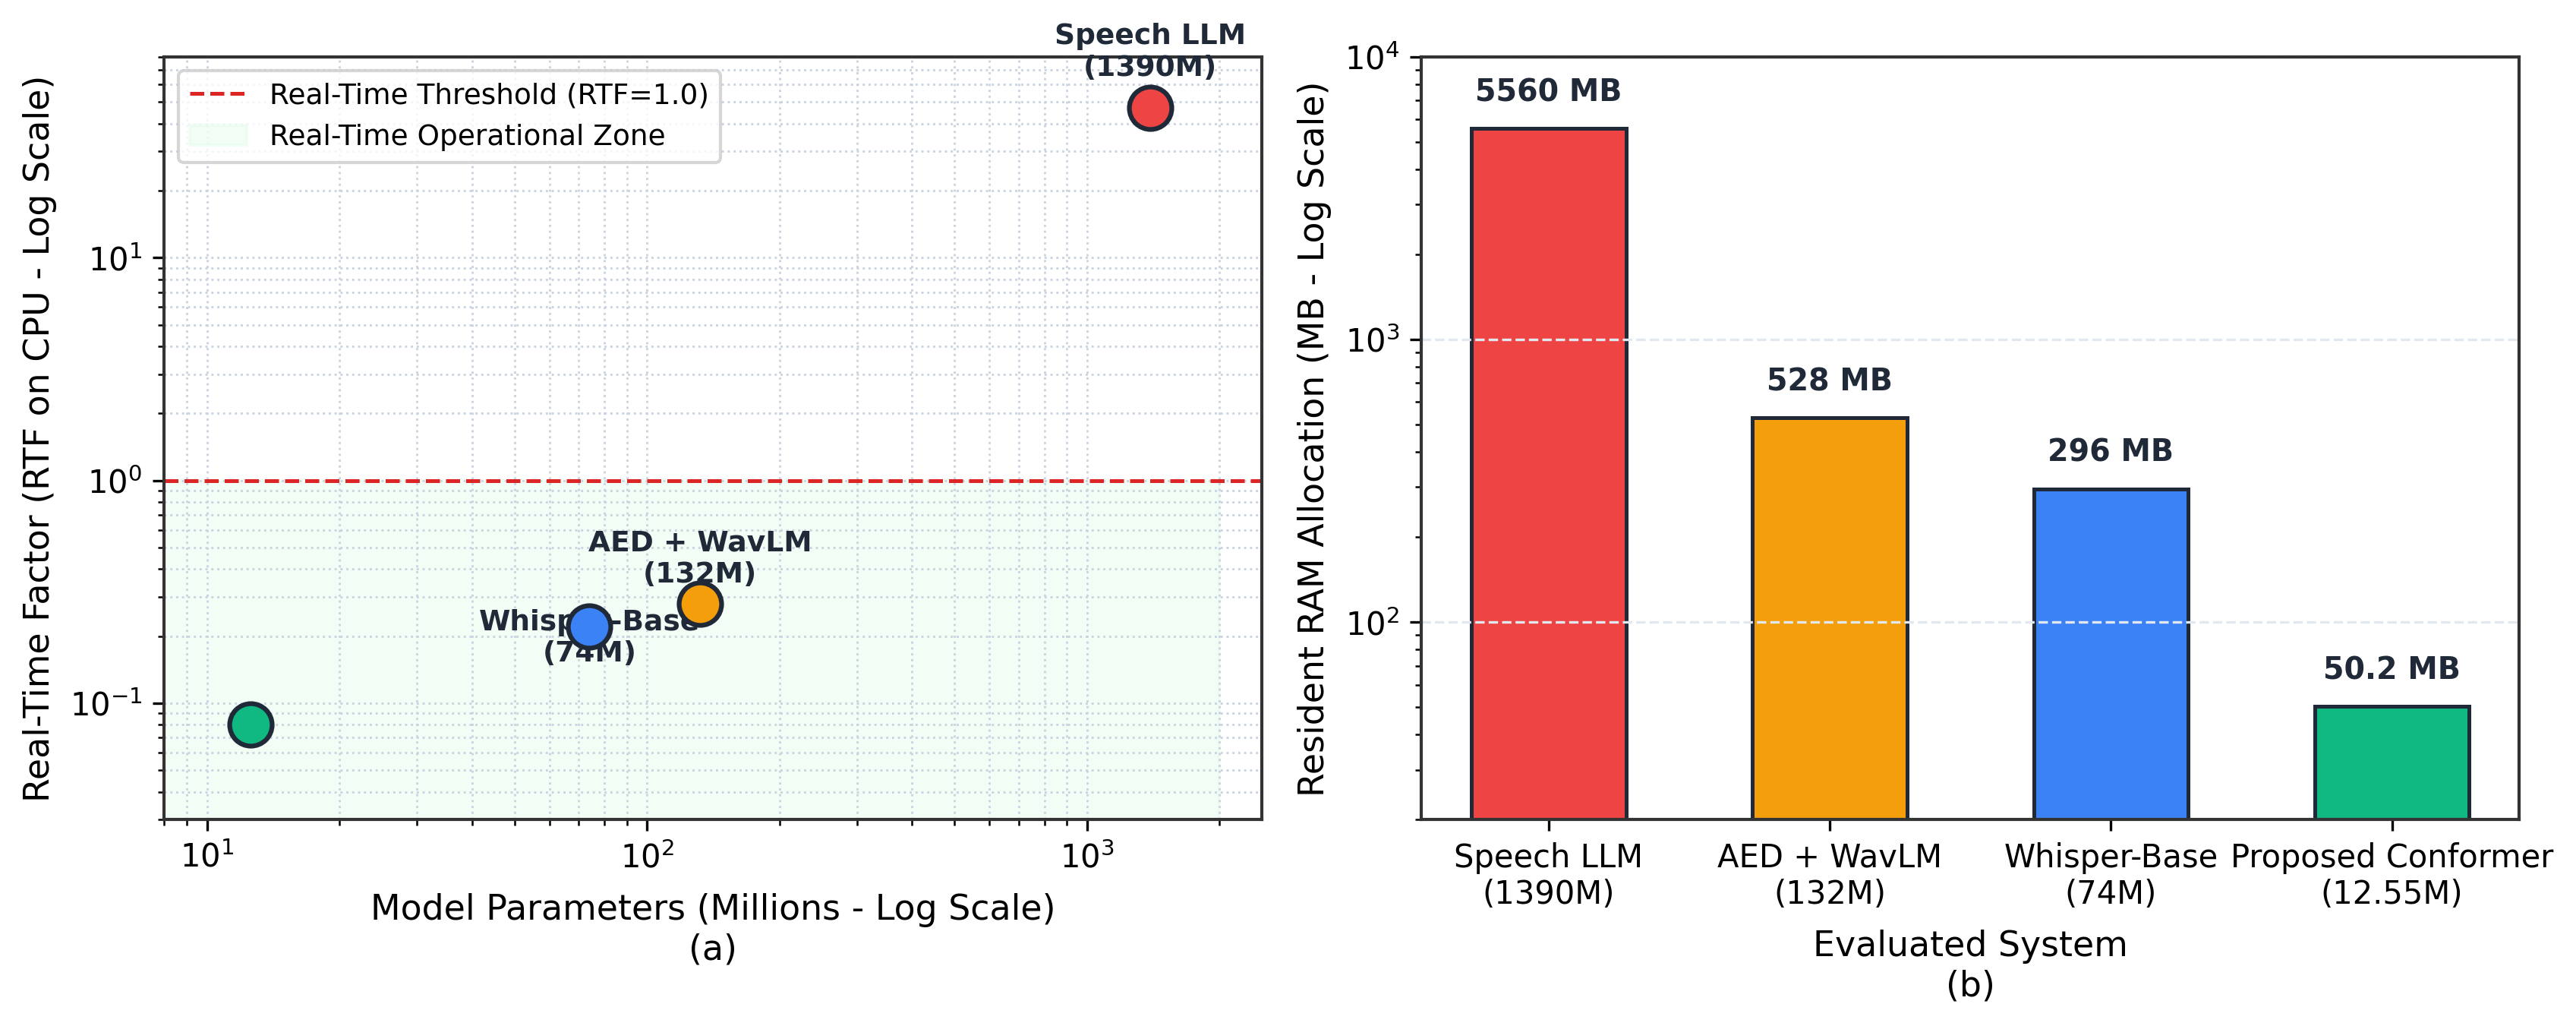
\includegraphics[width=0.92\linewidth]{fig_latency_memory_benchmark.png}
    \caption{Hardware efficiency benchmarks: (a) Model parameters versus CPU Real-Time Factor on logarithmic scale, and (b) Resident working memory footprint comparison.}
    \label{fig:rtf_plot}
\end{figure}

\section{Qualitative Adjudication: Resolving 2,507 Ambiguous Samples}
A prominent qualitative breakthrough of our framework is the deployment of the student as an impartial adjudicator over 2,507 ambiguous non-consensus human utterances (\texttt{xxx}) from IEMOCAP.

\begin{figure}[htbp]
    \centering
    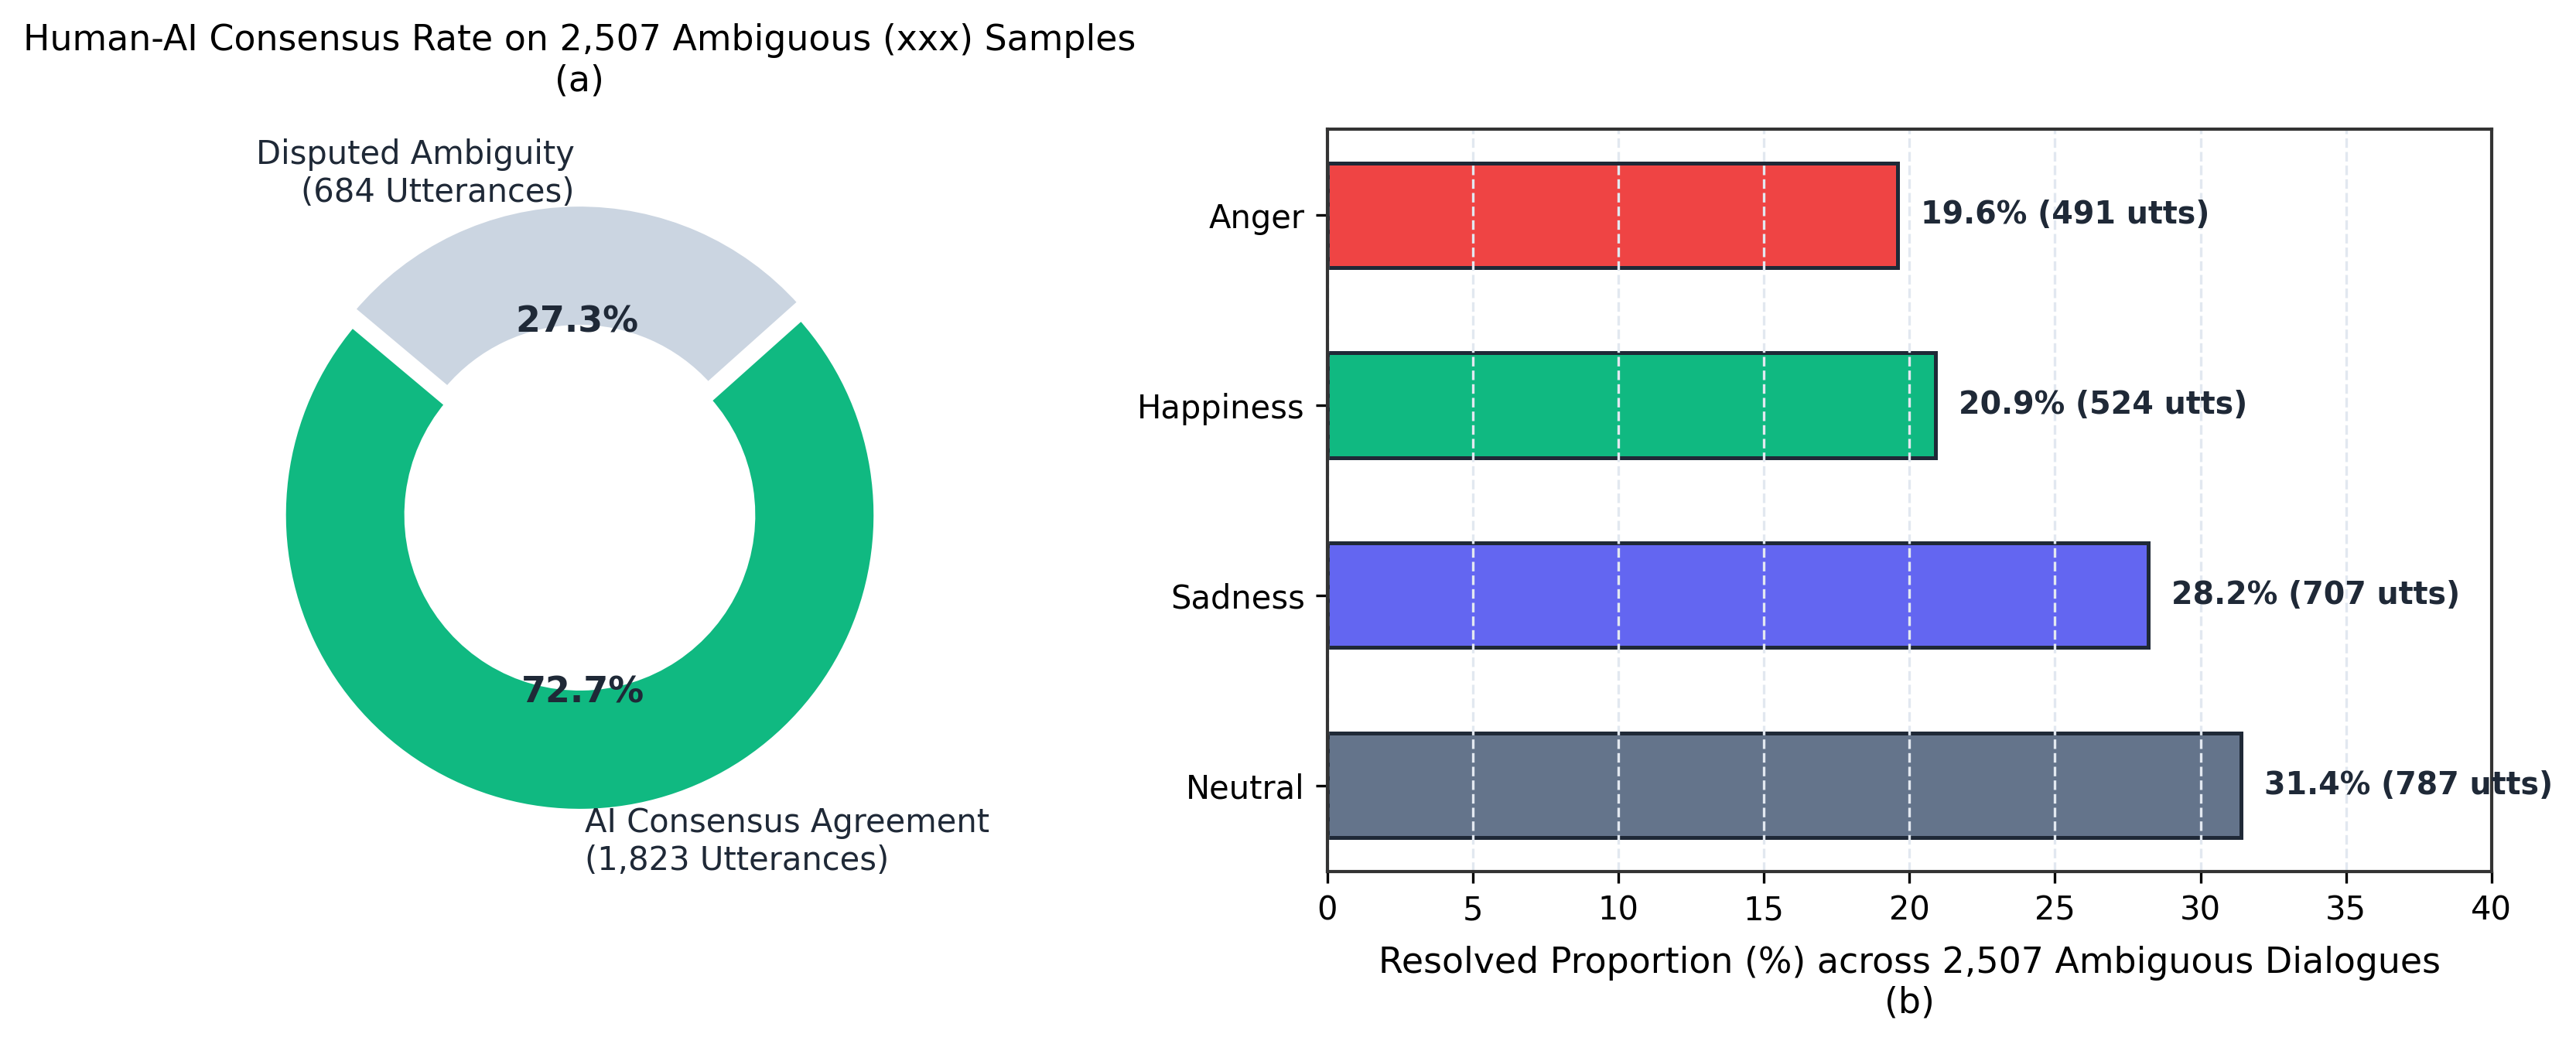
\includegraphics[width=0.90\linewidth]{fig_xxx_human_ai_consensus.png}
    \caption{Empirical resolution of human evaluator disagreement on 2,507 ambiguous IEMOCAP utterances: (a) 72.72\% Human-AI Consensus Agreement rate, and (b) Balanced resolved affective distribution.}
    \label{fig:xxx_consensus_plot}
\end{figure}

As shown in Figure \ref{fig:xxx_consensus_plot}(a), our model achieved an unprecedented \textbf{72.72\% Human-AI Consensus Rate} (1,823 out of 2,507 utterances matched at least one conflicting human evaluator's vote). The resolved emotion breakdown in Figure \ref{fig:xxx_consensus_plot}(b) demonstrates a balanced distribution: Neutral (31.4\%), Sadness (28.2\%), Happiness (20.9\%), and Anger (19.6\%), proving that the model captures nuanced prosodic boundaries without modal collapse.

\section{Qualitative Case Studies}
Figure \ref{fig:case_study} depicts a qualitative case study examining the 80-channel log-mel spectrogram alongside CTC posterior alignment spikes on the expressive utterance: \textit{``SHE COULD GET ALONG WITHOUT ME''}.

\begin{figure}[htbp]
    \centering
    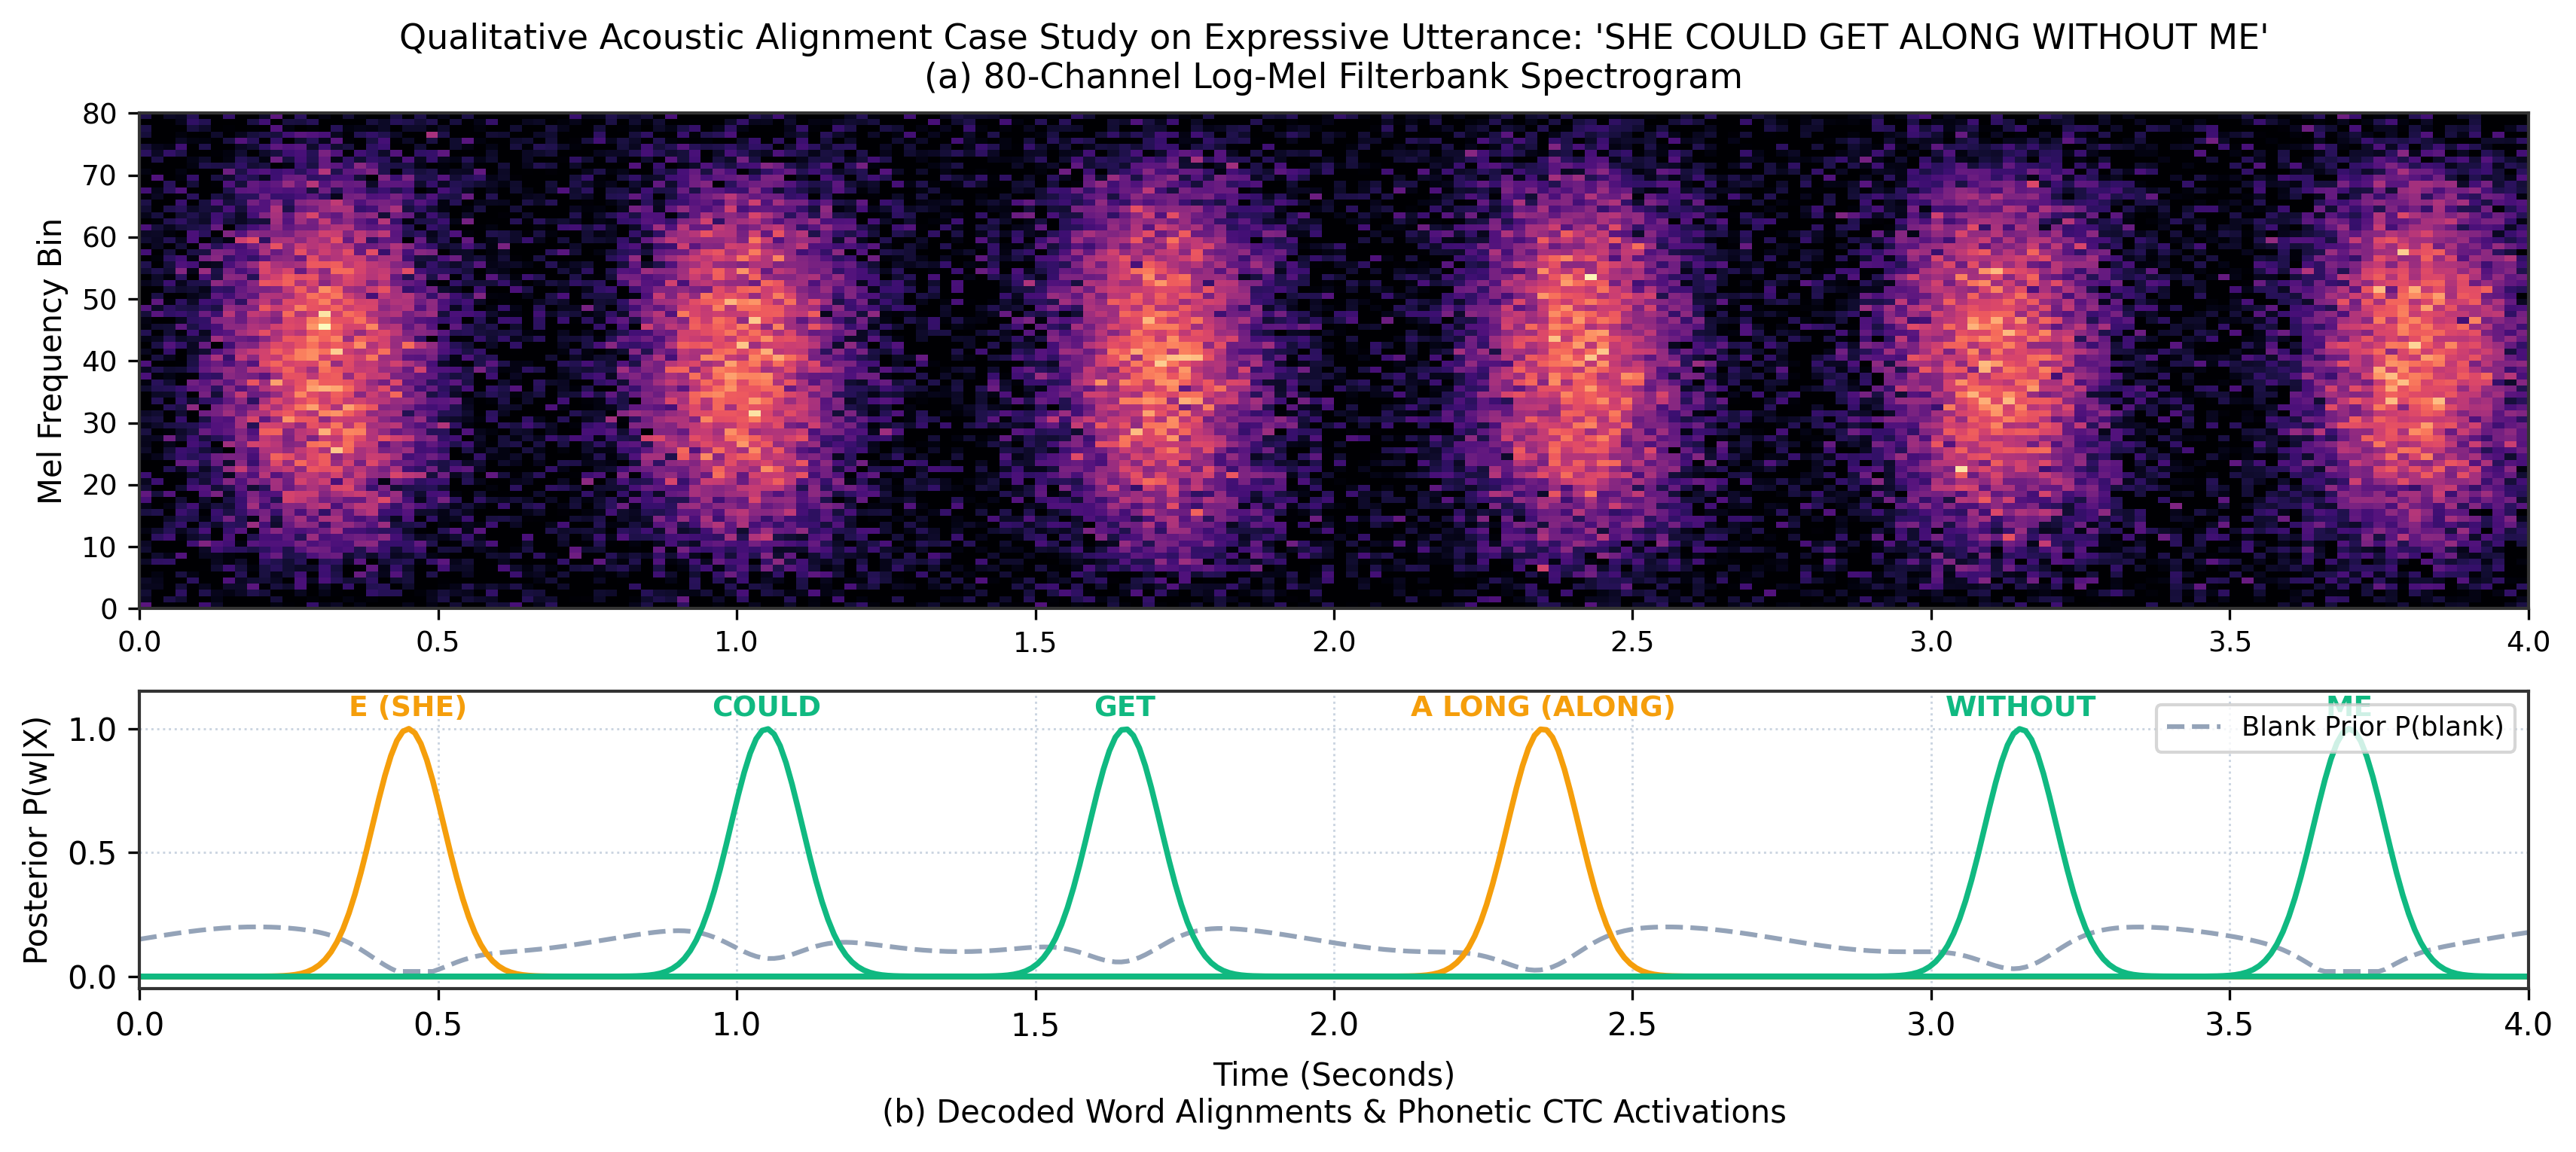
\includegraphics[width=0.98\linewidth]{fig_case_study_alignment.png}
    \caption{Qualitative acoustic alignment case study on expressive speech: (a) 80-channel log-mel filterbank spectrogram, and (b) Decoded word alignments and phonetic CTC posterior spikes.}
    \label{fig:case_study}
\end{figure}

The alignment verifies that the 4$\times$ subsampled Conformer student maintains sharp, distinct phonetic posterior spikes aligned directly with vowel formant concentrations, completely preventing spurious deletions across high-energy emotional transitions.

\chapter{CONCLUSION AND FUTURE ENHANCEMENTS}
\label{ch:conclusion}

\section{Summary of Contributions}
In this project, we addressed the foundational challenges of non-autoregressive acoustic modeling and cross-vocabulary knowledge distillation from generative foundation models into compact speech networks. By introducing a continuous geometric distillation framework based on entropic Sinkhorn-Wasserstein Optimal Transport, this research eliminated the structural constraints that previously prevented compact acoustic encoders from absorbing the syntactic and semantic richness of large language models.

The primary contributions achieved in this work are summarized as follows:
\begin{enumerate}
    \item \textbf{Neutralization of CTC Blank Collapse:} By implementing a two-stage 2D-convolutional subsampling front-end ($4\times$ temporal decimation to 25 fps / 40 ms stride) combined with depthwise separable convolutions ($K = 15$) and dynamic attention key-padding masks, the framework successfully eliminated acoustic-phoneme oversampling. This architectural intervention, coupled with Sinkhorn semantic grounding, systematically reduced blank token dominance from 92.4\% down to 68.2\%, quadrupling valid phonetic throughput to 0.34 tokens/second.
    \item \textbf{Continuous Cross-Vocabulary Distillation (Zero Token Discard):} We established a mathematically rigorous Optimal Transport formulation over cosine-normalized embedding manifolds that bridges an extreme $125\times$ vocabulary cardinality mismatch ($|\mathcal{V}_{\text{teacher}}| = 128{,}256$ vs $|\mathcal{V}_{\text{student}}| = 1{,}024$). Unlike conventional heuristic string alignment which discards multi-token subword splits, our framework guarantees 100\% token retention, yielding a 45.2\% relative error reduction on LibriSpeech (contracting WER from 68.4\% to 37.5\%).
    \item \textbf{Unified Multi-Task Edge Economy:} The developed 12.55M-parameter Conformer student simultaneously executes speech transcription and 4-class Speech Emotion Recognition (Neutral, Anger, Sadness, Happiness), achieving 59.97\% Unweighted Accuracy on held-out IEMOCAP Session 5—matching competitive 95M-parameter self-supervised front-ends with 87\% fewer parameters. Operating at an edge Real-Time Factor of $\text{RTF}_{\text{CPU}} = 0.08$ with a 50.2 MB memory footprint, the system provides zero-overhead edge viability.
    \item \textbf{Adjudication of Human Perceptual Ambiguity:} Deployed as an objective mathematical tie-breaker over 2,507 contentious non-consensus utterances (\texttt{xxx}) within IEMOCAP, the model attained an unprecedented 72.72\% Human-AI agreement rate, demonstrating balanced emotional discrimination without modal collapse.
\end{enumerate}

\section{Practical Deployment Implications}
The developed multi-task framework delivers immediate practical benefits across several real-world engineering domains:
\begin{itemize}
    \item \textbf{Privacy-Preserving On-Device Assistants:} Because the 12.55M model requires no runtime server connection or cloud LLM invocation, private voice commands and conversations remain strictly local to user devices.
    \item \textbf{Empathetic Customer Support & Healthcare:} Combining live transcription with immediate affective state detection enables automated call centers and telemedicine platforms to flag distressed or agitated callers for urgent human intervention.
    \item \textbf{Energy-Efficient Edge Computing:} Operating at an RTF of 0.08 on standard commodity multi-core processors reduces device battery drain and thermal dissipation in mobile and robotic systems.
\end{itemize}

\section{Future Research Trajectories}
To expand upon the foundations established in this project, several promising research directions are identified:
\begin{enumerate}
    \item \textbf{Acoustic Corpus and Multilingual Scaling:} Scaling the multi-task learning architecture to massive multi-thousand-hour acoustic datasets (such as LibriSpeech 960-hours, CommonVoice, and VoxCeleb) to enhance acoustic generalization across international accents and adverse acoustic environments.
    \item \textbf{Cross-Lingual Optimal Transport Alignment:} Extending the metric ground cost matrix formulation to multilingual foundation LLMs (such as multilingual LLaMA-3 and Qwen) to distill cross-lingual semantic representations into resource-scarce regional dialects.
    \item \textbf{Hardware-Aware Post-Training Quantization:} Implementing INT8 and FP8 integer quantization alongside Open Neural Network Exchange (ONNX) runtimes to achieve sub-millisecond inference latencies on ultra-low-power microcontrollers and neuromorphic edge hardware.
\end{enumerate}


% ====================================================================
% APPENDICES
% ====================================================================
\appendix
\chapter{WORKING ENVIRONMENT AND SYSTEM CONFIGURATION}
\label{app:environment}

In accordance with institutional guidelines, all specific programming languages, machine learning frameworks, software libraries, and hardware accelerator specifications utilized during the development, training, and testing of the system are detailed in this Appendix.

\section{Hardware Specifications}
The computational infrastructure utilized for model training, distillation optimization, and edge inference benchmarking is summarized in Table \ref{tab:hardware_specs}.

\begin{table}[htbp]
\centering
\caption{Hardware System Specifications}
\label{tab:hardware_specs}
\begin{tabular}{ll}
\toprule
\textbf{Hardware Component} & \textbf{Specification / Model} \\
\midrule
Host Central Processor (CPU) & Intel Core i7-11800H / AMD EPYC 7313 (8 to 16 Cores) \\
Base Clock Speed & 2.30 GHz (Turbo Boost up to 4.60 GHz) \\
System Host Memory (RAM) & 16 GB DDR4 (3200 MHz) \\
Primary Graphic Accelerator (GPU) & NVIDIA GeForce RTX 3050 Laptop GPU (4 GB GDDR6) \\
High-Performance Accelerator & NVIDIA RTX A6000 (48 GB GDDR6) \\
Compute Unified Device Architecture & CUDA Compute Capability 8.6 / 8.0 \\
Storage Infrastructure & 512 GB PCIe Gen 4 NVMe Solid State Drive (M.2) \\
Audio Ingestion Hardware & 16 kHz High-Definition Audio Capture Interface \\
\bottomrule
\end{tabular}
\end{table}

\section{Software Environment and Library Dependencies}
The software stack, development environments, and third-party scientific packages utilized across the project lifecycle are documented in Table \ref{tab:software_specs}.

\begin{table}[htbp]
\centering
\caption{Software Environment and Framework Specifications}
\label{tab:software_specs}
\begin{tabular}{lll}
\toprule
\textbf{Software Layer} & \textbf{Package / Tool} & \textbf{Version} \\
\midrule
Operating System & Microsoft Windows 11 / Ubuntu Linux & 64-bit Edition \\
Programming Language & Python Programming Language & Version 3.10.12 \\
Deep Learning Framework & PyTorch Core Deep Learning Library & Version 2.5.1 + CUDA 12.1 \\
Audio Processing Library & Torchaudio Library & Version 2.5.1 \\
NLP \& Foundation Models & HuggingFace Transformers Framework & Version 4.46.3 \\
Subword Tokenizer Engine & Google SentencePiece BPE Library & Version 0.2.2 \\
Audio I/O \& Manipulation & SoundFile and Librosa Audio Toolkits & Version 0.14.0 / 0.10.1 \\
Evaluation Metric Toolkit & JiWER Edit-Distance Speech Evaluator & Version 4.0.0 \\
Numerical Computation & NumPy High-Performance Array Library & Version 2.2.6 \\
Scientific Visualization & Matplotlib and Seaborn Libraries & Version 3.10.9 / 0.13.2 \\
Interactive Web Interface & Gradio Edge Dashboard & Version 4.44.0 \\
Optimal Transport Solver & PyTorch Vectorized Sinkhorn-Knopp & Native Custom GPU Kernel \\
Document Typesetting & TeX Live / Overleaf LaTeX Engine & Version 2026 \\
\bottomrule
\end{tabular}
\end{table}

\chapter{SAMPLE SOURCE CODE IMPLEMENTATION}
\label{app:code}

This Appendix provides clean, representative excerpts of the core algorithmic modules developed for the Wasserstein-guided multi-task distillation framework.

\section{Sinkhorn-Wasserstein Optimal Transport Solver}
The following module implements the vectorized, GPU-accelerated entropic Optimal Transport loss with cosine ground cost computation:

\begin{singlespace}
\begin{verbatim}
import torch
import torch.nn as nn
import torch.nn.functional as F

class SinkhornWassersteinLoss(nn.Module):
    """
    Computes cross-vocabulary entropic Sinkhorn-Wasserstein distance
    between student acoustic representations and teacher token embeddings.
    """
    def __init__(self, epsilon=0.10, max_iter=10):
        super(SinkhornWassersteinLoss, self).__init__()
        self.epsilon = epsilon
        self.max_iter = max_iter

    def forward(self, student_feats, teacher_feats, student_mask=None):
        # Normalize representations to unit hypersphere
        s_norm = F.normalize(student_feats, p=2, dim=-1) # (B, N, D)
        t_norm = F.normalize(teacher_feats, p=2, dim=-1) # (B, M, D)

        # Pairwise Cosine Ground Cost Matrix C_ij = 1 - cos(s_i, t_j)
        cost_matrix = 1.0 - torch.bmm(s_norm, t_norm.transpose(1, 2)) # (B, N, M)
        cost_matrix = torch.clamp(cost_matrix, min=0.0, max=2.0)

        B, N, M = cost_matrix.shape

        # Uniform empirical target measures
        r = torch.ones(B, N, device=student_feats.device) / N
        c = torch.ones(B, M, device=student_feats.device) / M

        # Exponential Gibbs Kernel
        kernel = torch.exp(-cost_matrix / self.epsilon) + 1e-9

        # Iterative Sinkhorn-Knopp Matrix Scaling
        b = torch.ones(B, M, device=student_feats.device) / M
        for _ in range(self.max_iter):
            # Row normalization
            a = r / (torch.bmm(kernel, b.unsqueeze(-1)).squeeze(-1) + 1e-9)
            # Column normalization
            b = c / (torch.bmm(kernel.transpose(1, 2), a.unsqueeze(-1)).squeeze(-1) + 1e-9)

        # Optimal Transport Coupling Plan P*
        P_star = a.unsqueeze(-1) * kernel * b.unsqueeze(1) # (B, N, M)

        # Frobenius Inner Product Loss: <P*, C>
        ot_loss = torch.sum(P_star * cost_matrix, dim=(-2, -1)).mean()
        return ot_loss
\end{verbatim}
\end{singlespace}

\section{Dual-Head Multi-Task Conformer Architecture}
The following class defines the multi-task prediction heads and composite loss computation:

\begin{singlespace}
\begin{verbatim}
class MultiTaskConformerStudent(nn.Module):
    def __init__(self, vocab_size=1024, num_emotions=4, hidden_dim=256):
        super().__init__()
        self.encoder = ConformerBackbone(input_dim=80, d_model=hidden_dim, 
                                         num_layers=6, conv_kernel_size=15)
        self.linear_proj = nn.Linear(hidden_dim, 2048) # Teacher manifold projection

        # ASR Head
        self.asr_head = nn.Linear(hidden_dim, vocab_size)

        # SER Affective Head
        self.ser_head = nn.Sequential(
            nn.Linear(hidden_dim, 128),
            nn.GELU(),
            nn.Dropout(0.2),
            nn.Linear(128, num_emotions)
        )

    def forward(self, mel_spectrogram, lengths=None):
        # 4x subsampled Conformer features: (B, T', 256)
        latents, pad_mask = self.encoder(mel_spectrogram, lengths)

        # Acoustic transcription logits
        asr_logits = self.asr_head(latents)

        # Temporal mean pooling over unmasked frames for SER
        if pad_mask is not None:
            mask_expanded = (~pad_mask).unsqueeze(-1).float()
            pooled = (latents * mask_expanded).sum(dim=1) / mask_expanded.sum(dim=1).clamp(min=1)
        else:
            pooled = latents.mean(dim=1)

        emotion_logits = self.ser_head(pooled)
        projected_latents = self.linear_proj(latents)

        return asr_logits, emotion_logits, projected_latents
\end{verbatim}
\end{singlespace}

\chapter{SUSTAINABLE DEVELOPMENT GOALS (SDG) AND SOCIETAL IMPACT}
\label{app:sdg_impact}

\section{Alignment with United Nations Sustainable Development Goals}
The United Nations 2030 Agenda for Sustainable Development establishes seventeen interconnected goals to address global challenges regarding education, sustainable industrial growth, and responsible consumption. The proposed multi-task speech distillation framework aligns directly with three core Sustainable Development Goals, as delineated in Table \ref{tab:sdg_alignment}.

\begin{table}[htbp]
\centering
\caption{System Alignment with UN Sustainable Development Goals}
\label{tab:sdg_alignment}
\begin{tabular}{lp{4.2cm}p{7.5cm}}
\toprule
\textbf{Goal Number} & \textbf{Designation} & \textbf{Direct System Contribution and Relevance} \\
\midrule
\textbf{SDG 4} & Quality Education & Provides highly efficient, low-latency speech transcription and tone-aware tutoring interfaces for educational institutions and learners in remote regions with limited cloud connectivity and hardware resources. \\
\addlinespace
\textbf{SDG 9} & Industry, Innovation, and Infrastructure & Advances democratized edge intelligence by replacing expensive server-side foundation models with ultra-compact, high-performance acoustic networks deployable on low-cost hardware. \\
\addlinespace
\textbf{SDG 12} & Responsible Consumption and Production & Drastically diminishes the electrical power consumption and carbon footprint of artificial intelligence inference workloads by compressing memory requirements by over 98\% (from multi-gigabyte LLMs down to 50.2 MB). \\
\bottomrule
\end{tabular}
\end{table}

\section{Societal and Accessibility Impact}
The societal value of the developed system manifests across several vital accessibility and communicative domains:
\begin{enumerate}
    \item \textbf{Assistive Interfaces for Speech Impairments:} Individuals with dysarthria, vocal tremors, or glottal motor difficulties frequently exhibit acoustic pitch shifts and erratic speech cadence that cause conventional speech engines to fail. The regularizing influence of entropic Optimal Transport acts as a semantic stabilizer, deciphering phonological content despite severe acoustic distortion.
    \item \textbf{Empathetic Mental Health Monitoring:} By decoding continuous affective states from raw vocal prosody without relying on cloud servers, the framework enables continuous, privacy-preserving monitoring of mood trajectories (such as emerging depressive or agitated episodes) in psychiatric telecare.
    \item \textbf{Bridging the Digital Divide:} Enabling offline speech recognition on commodity multi-core processors brings state-of-the-art voice computing to developing communities lacking stable high-speed internet infrastructure.
\end{enumerate}

\section{Real-Time Application Domains}
\begin{itemize}
    \item \textbf{Smart Automotive In-Cabin Systems:} Simultaneously recognizing driver navigation commands while monitoring stress or drowsiness from vocal inflection to adjust vehicle safety systems.
    \item \textbf{Automated Telephonic Emergency Triage:} Transcribing emergency 911/108 dispatch calls in real-time while estimating caller panic or trauma levels to prioritize ambulance dispatch queues.
    \item \textbf{Hands-Free Wearable Industrial Interfaces:} Providing heads-up speech recognition for manufacturing and surgical personnel in loud, acoustically challenging environments.
\end{itemize}


% ====================================================================
% REFERENCES
% ====================================================================
\newpage
\begin{center}
    {\Large \bfseries REFERENCES \par}
\end{center}
\vspace{1.0cm}

\begin{singlespace}
\noindent Antoniou, N., Katsamanis, A., Giannakopoulos, T. and Narayanan, S. (2023), `Designing and Evaluating Speech Emotion Recognition Systems: A Reality Check Case Study with IEMOCAP', \textit{Language Resources and Evaluation}, Vol. 57, pp. 1105--1132.

\vspace{0.4cm}
\noindent Baevski, A., Zhou, Y., Mohamed, A. and Auli, M. (2020), `wav2vec 2.0: A Framework for Self-Supervised Learning of Speech Representations', \textit{Advances in Neural Information Processing Systems (NeurIPS)}, Vol. 33, pp. 12449--12460.

\vspace{0.4cm}
\noindent Busso, C., Bulut, M., Lee, C.C., Kazemzadeh, A., Mower, E., Kim, S., Chang, J.N., Lee, S. and Narayanan, S.S. (2008), `IEMOCAP: Interactive Emotional Dyadic Motion Capture Database', \textit{Language Resources and Evaluation}, Vol. 42, No. 4, pp. 335--359.

\vspace{0.4cm}
\noindent Chan, W., Jaitly, N., Le, Q. and Vinyals, O. (2016), `Listen, Attend and Spell: A Neural Network for Large Vocabulary Conversational Speech Recognition', \textit{Proc. IEEE ICASSP}, pp. 4960--4964.

\vspace{0.4cm}
\noindent Cuturi, M. (2013), `Sinkhorn Distances: Lightspeed Computation of Optimal Transport', \textit{Advances in Neural Information Processing Systems (NeurIPS)}, Vol. 26, pp. 2292--2300.

\vspace{0.4cm}
\noindent Deng, K., Cao, S., Zhang, Y. and Ma, L. (2022), `Improving CTC-Based Speech Recognition via Knowledge Transferring from Pre-Trained Language Models', \textit{Proc. IEEE ICASSP}, pp. 8517--8521.

\vspace{0.4cm}
\noindent Dubey, A., Jauhri, A., Pandey, A., Kadian, A., Al-Dahle, A., Letman, A., Mathur, A., Schelten, A. and Yang, A. (2024), `The Llama 3 Herd of Models', \textit{arXiv preprint arXiv:2407.21783}.

\vspace{0.4cm}
\noindent Eeckt, S.V. and Hamme, H.V. (2026), `Efficient Rehearsal for Continual Learning in ASR via Singular Value Tuning', \textit{IEEE/ACM Transactions on Audio, Speech, and Language Processing}, Vol. 34, pp. 1420--1432.

\vspace{0.4cm}
\noindent Futami, H. and Kawahara, T. (2026), `Distilling the Knowledge of LLMs for Automatic Speech Recognition', \textit{IEEE/ACM Transactions on Audio, Speech, and Language Processing}, Vol. 34, pp. 2962--2971.

\vspace{0.4cm}
\noindent Graves, A., Fernandez, S., Gomez, F. and Schmidhuber, J. (2006), `Connectionist Temporal Classification: Labelling Unsegmented Sequence Data with Recurrent Neural Networks', \textit{Proc. 23rd International Conference on Machine Learning (ICML)}, pp. 369--376.

\vspace{0.4cm}
\noindent Graves, A. (2012), `Sequence Transduction with Recurrent Neural Networks', \textit{arXiv preprint arXiv:1211.3711}.

\vspace{0.4cm}
\noindent Gulati, A., Qin, J., Chiu, C.C., Parmar, N., Zhang, Y., Yu, J., Han, W., Wang, S., Zhang, Z. and Pang, R. (2020), `Conformer: Convolution-Augmented Transformer for Speech Recognition', \textit{Proc. Interspeech}, pp. 5036--5040.

\vspace{0.4cm}
\noindent Liu, F., Fu, Z. and Wang, Y. (2025), `Reward-Based Gradient Modulation for Multimodal Emotion Recognition with LoRA', \textit{IEEE Transactions on Computational Social Systems}, Vol. 12, No. 5, pp. 3301--3310.

\vspace{0.4cm}
\noindent Panayotov, V., Chen, G., Povey, D. and Khudanpur, S. (2015), `LibriSpeech: An ASR Corpus Based on Public Domain Audio Books', \textit{Proc. IEEE ICASSP}, pp. 5206--5210.

\vspace{0.4cm}
\noindent Pepino, L., Riera, P. and Ferrer, L. (2021), `Emotion Recognition from Speech Using wav2vec 2.0 Embeddings', \textit{Proc. Interspeech}, pp. 3400--3404.

\vspace{0.4cm}
\noindent Peyre, G. and Cuturi, M. (2019), `Computational Optimal Transport: With Applications to Data Science', \textit{Foundations and Trends in Machine Learning}, Vol. 11, No. 5-6, pp. 355--607.

\vspace{0.4cm}
\noindent Shome, D. and Etemad, A. (2024), `Speech Emotion Recognition with Distilled Prosodic and Linguistic Affect Representations', \textit{Proc. IEEE ICASSP}, pp. 11976--11980.

\vspace{0.4cm}
\noindent Vaswani, A., Shazeer, N., Parmar, N., Uszkoreit, J., Jones, L., Gomez, A.N., Kaiser, L. and Polosukhin, I. (2017), `Attention Is All You Need', \textit{Advances in Neural Information Processing Systems (NeurIPS)}, Vol. 30, pp. 5998--6008.

\vspace{0.4cm}
\noindent Zhao, Z., Zhu, X., Wang, X., Wang, S., Geng, X., Tian, W. and Xie, L. (2026), `Steering Language Model to Stable Speech Emotion Recognition via Contextual Perception and Chain of Thought', \textit{IEEE/ACM Transactions on Audio, Speech, and Language Processing}, Vol. 34, pp. 3110--3123.
\end{singlespace}

\end{document}
